% Scientific content frozen 6 October 2026; 

\documentclass[aps,pra,reprint,superscriptaddress,longbibliography]{revtex4-2}
\usepackage{amsmath,amssymb,bm,mathtools}
\usepackage{booktabs}
\usepackage{pgfplots}
\pgfplotsset{compat=1.18}
\usepackage[colorlinks=true,citecolor=blue,urlcolor=blue,linkcolor=blue]{hyperref}
\newcommand{\dd}{\mathrm d}
\newcommand{\Tr}{\operatorname{Tr}}
\newcommand{\Var}{\operatorname{Var}}
\newcommand{\Wd}{W_{\mathrm{diss}}}
\newcommand{\E}{\mathbb E}
\newcommand{\Prob}{\mathbb P}
\newcommand{\calE}{\mathcal E}
\newcommand{\calB}{\mathcal B}
\newcommand{\R}{\mathbb R}
\newcommand{\norm}[1]{\left\lVert#1\right\rVert}
\newcommand{\sinc}{\operatorname{sinc}}
\begin{document}
\title{Microscopic work under stationary boundary calibration}
\author{R. Arun Chandru}
\email{arun.chandru@gmail.com}
\date{\today}
\begin{abstract}
Calibrating a confining wall at low energies does not specify the work of changing its microscopic profile. We quantify this distinction using positive finite potentials on a fixed Hilbert space and complete thermal initial states. For any fixed finite order of the wall's energy-dependent boundary response, a nonconstant finite-time drive can preserve that response throughout its motion while producing a strictly positive leading dissipated-work coefficient. The physical duration scales with the inverse wall height. A complete off-label transition law resolves rare outcomes of probability of order $r^3$ at energies of order $r^{-2}$, giving mean dissipation of order $r$ and variance of order $r^{-1}$. For sudden changes in arbitrary smooth bounded cavities, the leading work coefficients factor into thermal boundary pressure and microscopic profile energies. This factorization extends to canonical ideal Bose and Fermi gases at fixed particle number. A smooth, scalar-calibrated finite-wall example certifies positive dissipation and a bounded-energy detection event at nonzero duration, including full thermal tails and finite reporting errors. The preparation costs distinguish observing a rare event from estimating its moments. These results specify the dynamical information left outside stationary boundary calibration without implying a resource-free sensing advantage.
\end{abstract}
\maketitle

\section{Introduction}

A high confining potential is often replaced by a boundary condition. This replacement is useful because low-energy particles primarily resolve a small set of boundary-response coefficients rather than the detailed shape of the barrier. A separate question arises when the barrier itself is changed: how much of the resulting work distribution is fixed by those same coefficients? The question concerns an intervention on a physical potential, not simply the precision of a spectral fit.

Quantum work statistics distinguish energy eigenvalues from transition probabilities \cite{Talkner,Campisi}. Supersymmetric quenches have nontrivial work distributions despite closely related spectra \cite{CampbellQuench}, and finite-time control can distinguish states with the same instantaneous energy \cite{CampbellControl}. Local potential quenches also have established ultraviolet singularities in their work moments \cite{Sindona}. Thus the general observation that stationary spectral information need not determine driven behavior is not, by itself, a new principle. The issue addressed here is a more constrained physical realization: a positive local wall, an unchanged free interior, fixed microscopic profiles, an exact prescribed finite boundary calibration, and the complete thermal work law generated by changing that wall.

The static approximation has substantial antecedents. Large-coupling spectral theory gives finite-barrier boundary layers, resolvent corrections and normal-derivative eigenvalue shifts \cite{BruneauCarbou,Nguyen,HintzMoser}; Robin asymptotics provide a related boundary description \cite{Ognibene}. The normal-derivative sum appearing in a thermal shape derivative is an established pressure quantity \cite{ElSoufi}. These results identify the correct stationary scale. Work moments require additional control: the initially populated spectrum is infinite, and rare final high-energy states cannot be dropped simply because individual low eigenvalues are accurately approximated.

A related finite-wall analysis treats changes of wall height under a bounded-action control budget \cite{ChandruRare}. There the boundary extrapolation length changes: label-changing probability is of order $r^2$, while the leading energetic cost is carried by a rarer order-$r^3$ sector. Here the stationary response is deliberately matched. The endpoint difference becomes square integrable in the boundary coordinate, the order-$r^2$ contribution disappears, and the entire label-changing probability joins the order-$r^3$ limiting law. The earlier control-uniform obstruction does not transfer to this calibrated problem. We instead construct nonzero drives inside finite-order calibration level sets and prove their work laws for fixed microscopic duration.

We connect these two questions in the same finite-potential operators. There are two complementary results. In one dimension, every prescribed finite order of stationary boundary response can remain exactly fixed along a nonconstant drive, yet the drive has a positive leading energetic cost. A limiting transition measure gives the full rare-event probability and its first two energy moments. In a general smooth cavity, a sudden profile change has a simpler geometry--profile factorization: thermal boundary pressure supplies the geometric and statistical weight, while two profile energies determine dissipation and variance. Fixed-particle ideal quantum statistics changes the pressure, but not these microscopic functionals. Identical-particle work distributions are already developed \cite{Gong}; the additional statement here is their calibrated finite-wall asymptotic, with the canonical pair contribution controlled on the same scale.

The distinction has a concrete finite-parameter test. We construct a smooth positive path whose zero-energy wall response is constant at every instant, enclose its exact thermal work quantities, and certify a finite-band positive-work event at nonzero driving time. No final-state spectral cutoff is used to establish the certificate. A comparison across selected thermal and canonical preparations tests the pressure-normalized ratio at finite wall thickness. Detection and moment-estimation costs are stated separately, and a constrained profile comparison improves a sufficient detection guarantee without asserting that it globally optimizes the unknown true probability.

The boundary calibration in this paper always means the specified low-energy response coefficients. It does not mean complete stationary states, all stationary observables, or equality of the full finite-wall spectra. Likewise, the finite-time asymptotic resolves the microscopic time scale; it is not a fixed laboratory-duration limit. These distinctions are central to the physical interpretation rather than qualifications added after the calculation.

\section{A physical wall and its stationary calibration}

Use a length unit $L$, energy unit $E_L=\hbar^2/(2mL^2)$ and time unit $\hbar/E_L$. Energies, times and inverse temperature $\beta$ below are dimensionless. A particle occupies the fixed interval $(0,1+b)$, with $b>0$ and Dirichlet conditions at the two outer endpoints. The interior $(0,1)$ is free. A wall profile $V$ defines
\begin{equation}
 H_{V,r}=-\partial_y^2+r^{-2}\mathbf1_{y>1}V((y-1)/r),
 \qquad r>0.\label{eq:interval}
\end{equation}
The profile is real, bounded and $C^2$ on $[0,\infty)$, is strictly positive, and equals a positive constant beyond a fixed distance. All profiles, geometry and temperature are fixed before $r\downarrow0$. The wall height and transition width scale together. At every positive $r$, the potential is finite and the Hilbert space and operator domain are unchanged.

Let $w_V$ be the decaying solution of
\begin{equation}
 -w_V''+Vw_V=0,\qquad w_V(0)=1,
 \qquad h_V=-w_V'(0)>0.\label{eq:wallsolution}
\end{equation}
The energy-dependent response $h_V(E)$ is defined similarly for $-w''+Vw=Ew$, with the decaying normalization near $E=0$. Positivity gives an analytic neighborhood of zero. Matching through order $J$ means equality of $h_V^{(j)}(0)$ for $0\le j\le J$. The corresponding physical extrapolation length at leading order is $r/h_V$.

The initial state is the complete Gibbs state $\rho_{0,r}=e^{-\beta H_{0,r}}/Z_{0,r}$. For endpoint eigenpairs $(e_{j,n},\phi_{j,n})$ and unitary evolution $\mathcal U_r$, the two-energy-measurement law is
\begin{equation}
 p_{n,m}=\frac{e^{-\beta e_{0,n}}}{Z_{0,r}}
       |\langle\phi_{1,m},\mathcal U_r\phi_{0,n}\rangle|^2,
 \qquad W=e_{1,m}-e_{0,n}.\label{eq:tpm}
\end{equation}
Write $\Delta F_r=-\beta^{-1}\log(Z_{1,r}/Z_{0,r})$ and $\Wd=\E W-\Delta F_r$. Dissipated work is not heat delivered to a bath during the isolated evolution. The standard entropy identity is
\begin{equation}
 \beta\Wd=D(\mathcal U_r\rho_{0,r}\mathcal U_r^*\Vert\rho_{1,r}),
 \label{eq:entropy}
\end{equation}
with the pre-final-measurement state on the left of the relative entropy \cite{Deffner}. Only for a sudden change may it be replaced by $\rho_{0,r}$.

For the hard-wall interior, put $\lambda_n=(n\pi)^2$ and
\begin{equation}
 U_D(\beta)=\frac{\sum_{n\ge1}\lambda_ne^{-\beta\lambda_n}}
                         {\sum_{n\ge1}e^{-\beta\lambda_n}},
 \qquad C_\beta=\frac{2U_D(\beta)}{h^2}.\label{eq:pressure1d}
\end{equation}
If $h_{V_0}=h_{V_1}=h$, the endpoint eigenvalue differences are $O(r^3)$ for each fixed label. Matching through order $J$ strengthens this to $O(r^{2J+3})$, and the same order holds for the full log-partition-function difference. The constants depend on the fixed profiles and $J$; the assertion is not uniform as $J$ grows. The spectral estimates and their thermal summation are derived below.

\section{Work left outside the calibration}

First consider a sudden change between two profiles with common $h$. Define on the positive half-line
\begin{equation}
 \begin{gathered}
 u=w_0-w_1,\qquad f=(V_1-V_0)w_0,\\
 \calE_1(v)=\int_0^\infty(|v'|^2+V_1|v|^2)\,\dd z.
 \end{gathered}
 \label{eq:mismatch}
\end{equation}
Both $u(0)$ and $u'(0)$ vanish. Its zero extension therefore lies in the domain of the actual limiting full-line operator
\begin{equation}
 A_1=-\partial_z^2+\mathbf1_{z>0}V_1(z),\qquad A_1u=f.
 \label{eq:fullop}
\end{equation}
This square-integrable cancellation is stronger than a formal use of a zero-energy resolvent. It produces
\begin{align}
 \frac{\Wd}{r}&\longrightarrow C_\beta\calE_1(u),\label{eq:suddenmean}\\
 r\Var W&\longrightarrow C_\beta\norm{f}_2^2,\label{eq:suddenvar}\\
 r^{-3}\Prob(m\ne n)&\longrightarrow C_\beta\norm{u}_2^2.
 \label{eq:suddenprob}
\end{align}
All coefficients are positive for distinct profiles. The leading mean cost tends to zero, whereas the variance diverges. The probability in Eq.~\eqref{eq:suddenprob} is a change of ordered spectral label, not the probability of nonzero work: typical same-label outcomes generally have small but nonzero work because the finite-wall spectra are not identical.

The scales have a direct boundary interpretation. A normalized low-energy orbital has amplitude of order $r$ in a layer of width $r$. Matching $h$ cancels the larger change of the interior orbital; the surviving wall difference therefore has squared norm of order $r^3$. Its variation occurs on length $r$, so its outgoing energy scale is $r^{-2}$. Multiplying the probability by one or two powers of that energy gives the orders $r$ and $r^{-1}$. The analysis below proves this explanation for the entire thermal preparation and controls the energy tails that this scale argument alone would not justify.

More precisely, if $\mu_u^{A_1}(S)=\langle u,\mathbf1_S(A_1)u\rangle$, then
\begin{equation}
 r^{-3}\Prob(r^2W\in\dd E,\ m\ne n)
       \ \Longrightarrow\ C_\beta\,\dd\mu_u^{A_1}(E).
 \label{eq:suddenlaw}
\end{equation}
The total masses and the first two energy-weighted totals converge. There is no discarded contribution at zero, infinity or negative work. The limiting measure assigns its full mass to positive energies, although zero can belong to its closed support. This is what allows the same rare-event description to account for probability, mean work and variance, rather than deriving divergent moments from unweighted weak convergence.

\subsection{Keeping the calibration fixed during the drive}

Let $V_s$, $0\le s\le1$, be a $C^1$ path in $L^\infty$ of bounded potentials with uniformly bounded spatial $C^2$ norms and a common positive constant tail. Drive Eq.~\eqref{eq:interval} at $s=t/(\eta r^2)$, with fixed $0<\eta<\infty$. The endpoint response is matched. Let $U(s,t)$ propagate $A_s=-\partial_z^2+\mathbf1_{z>0}V_s$ according to $i\partial_sU(s,t)=\eta A_sU(s,t)$. With $\widehat w_0=\mathbf1_{z>0}w_0$, define square-integrable vectors
\begin{align}
 q_s&=-i\eta\int_0^s U(s,t)(V_t-V_0)_+\widehat w_0\,\dd t,
       \label{eq:q}\\
 d&=u+q_1,\nonumber\\
 g&=\int_0^1U(1,s)\dot V_{s,+}(\widehat w_0+q_s)\,\dd s.
       \label{eq:g}
\end{align}
Here a subscript $+$ means extension by zero to the left, not a positive part. No propagator is applied to a nonnormalizable stationary state. Actual finite-interval graph convergence gives $d\in D(A_1)$ and $A_1d=g$. Equations~\eqref{eq:suddenprob} and \eqref{eq:suddenlaw} then hold with $u$ replaced by $d$, and Eqs.~\eqref{eq:suddenmean}--\eqref{eq:suddenvar} with $\calE_1(u)$ and $\norm f^2$ replaced by $\langle d,A_1d\rangle$ and $\norm{A_1d}^2$.

If $h_s=h$ throughout the path, the same vector has the useful representation
\begin{equation}
 d=-\int_0^1U(1,s)\dot w_s\,\dd s,\label{eq:tangentdrive}
\end{equation}
where $\dot w_s$ is extended by zero. Thus the dynamical excitation samples directions of microscopic change that a fixed boundary response leaves available.

This freedom persists at every prescribed finite calibration order. For each fixed $J$ and fixed finite $\eta$, one can choose a nonconstant positive path satisfying
\begin{equation}
 h_{V_s}^{(j)}(0)=h_{V_0}^{(j)}(0),
 \quad 0\le j\le J,\quad 0\le s\le1,\label{eq:jet}
\end{equation}
such that $d\ne0$. Its instantaneous thermal free energy changes by only $O(r^{2J+3})$, uniformly along the path, while its work coefficients in the preceding limits are positive. The amplitude may depend on $J$ and $\eta$, and is then fixed before $r\downarrow0$.

The construction is explicit in its mechanism. At a constant profile, perturbing $V$ by a compact bump changes the response by
\begin{equation}
 \delta h(E)=\int_0^\infty e^{-2\sqrt{1-E}z}\delta V(z)\,\dd z.
 \label{eq:variationh}
\end{equation}
The first $J+1$ Taylor kernels are an exponential times independent polynomials. Choosing $J+2$ disjoint narrow bumps gives a rank-$J+1$ calibration map and a nontrivial local curve in its level set. If $v$ is the nonzero derivative of the normalized wall solution along this curve, a small fixed amplitude $\delta$ gives
\begin{equation}
 d_\delta=-\delta e^{-i\eta A_0/2}\sinc(\eta A_0/2)v
                      +O_\eta(\delta^2)\quad\text{in }D(A_0).
 \label{eq:filter}
\end{equation}
The multiplier vanishes only at discrete positive energies. Since the full-line positive wall has no eigenvalues, it cannot annihilate a nonzero $v$. This supplies positivity at every fixed finite $\eta$ without assuming that all nonconstant paths excite the system.

\section{A pressure--profile law beyond one dimension}

Let $\Omega\subset\R^d$ be any fixed bounded smooth connected cavity. Let $\Gamma$ be a nonempty union of complete boundary components. Attach a fixed smooth normal collar outside $\Gamma$ and impose Dirichlet conditions at the outer enclosure and on the uncontrolled components. The normal distance is $t(x)$ and the actual exterior potential is $r^{-2}V(t(x)/r)$. A bounded enclosure is essential: a constant finite plateau throughout unbounded exterior space would not have a finite Gibbs partition function.

For Dirichlet eigenpairs $(\lambda_n,\phi_n)$ in $\Omega$, define the integrated thermal boundary pressure
\begin{equation}
 \calB_\Omega(\beta)=\frac1{Z_D}\sum_n e^{-\beta\lambda_n}
             \int_\Gamma |\partial_\nu\phi_n|^2\,\dd S.
 \label{eq:boundarypressure}
\end{equation}
The sum is basis independent through degenerate eigenspaces. For a ball of radius $R$, the Rellich identity gives $\calB_\Omega=2U_D/R$. For the interval with only its right endpoint controlled it is $2U_D$, not the $4U_D$ associated with controlling both endpoints.

The finite-potential thermal trace obeys, for every fixed admissible profile and fixed smooth bounded eventually constant $F$,
\begin{equation}
 r^{-3}\Tr\rho_{V,r}\mathbf1_{\rm collar}F(t/r)
   \longrightarrow\frac{\calB_\Omega}{h_V^2}
             \int_0^\infty Fw_V^2\,\dd z.\label{eq:localtrace}
\end{equation}
This is a complete trace statement, not a fixed-mode boundary-layer replacement. The proof below combines an actual-wall resolvent expansion, an all-index eigenvalue bound and a convexity argument that does not differentiate an uncontrolled remainder.

For matched $h_0=h_1=h$, Eq.~\eqref{eq:localtrace} yields
\begin{equation}
 \frac{\Wd}{r}\longrightarrow\frac{\calB_\Omega}{h^2}\calE_1(u),
 \qquad r\Var W\longrightarrow\frac{\calB_\Omega}{h^2}\norm f^2.
 \label{eq:geometricwork}
\end{equation}
Curvature and degeneracies do not change this leading factorization. This result concerns sudden moments. It does not assert a higher-dimensional complete off-label law, arbitrary-order curved-boundary calibration, or a finite-time result for arbitrary geometry.

\subsection{Imperfect calibration and an energy interpretation}

The factorization has a useful formulation even when $h_0\ne h_1$. Set
\begin{equation}
 a=\frac{w_0}{h_0}-\frac{w_1}{h_1},\qquad
 L_1=-\partial_z^2+V_1\quad\text{on }(0,\infty),\; a'(0)=0.
 \label{eq:neumannmismatch}
\end{equation}
The positive half-line operator $L_1$ has Neumann boundary condition. The mismatch belongs to its domain and $L_1a=f/h_0$. Integration by parts gives
\begin{equation}
 \calE_1(a)=\frac1{h_0^2}\int(V_1-V_0)w_0^2\,\dd z
                          -\frac1{h_0}+\frac1{h_1}.\label{eq:unmatchedenergy}
\end{equation}
Consequently the complete sudden limits take the unified form
\begin{equation}
 \frac{\Wd}{r}\to\calB_\Omega\calE_1(a),\qquad
 r\Var W\to\calB_\Omega\norm{L_1a}^2.\label{eq:unified}
\end{equation}
For a nonzero intervention, the normalized ratio therefore satisfies
\begin{equation}
 \frac{r^2\Var W}{\Wd}\longrightarrow
 \frac{\norm{L_1a}^2}{\langle a,L_1a\rangle}
                       \ge\inf_{z\ge0}V_1(z)>0.
 \label{eq:ratio}
\end{equation}
It is an energy average in the auxiliary Neumann spectral measure weighted by energy. This interpretation does not identify that measure with the actual full-line outgoing work law, nor impose a positive lower threshold on every measured work outcome.

The unscaled variance-to-dissipation ratio is a familiar work Fano factor. Generalized linear-response theory expresses work cumulants through a common relaxation function \cite{Guarnieri}; its application to inhomogeneous many-body systems includes this ratio \cite{Palamara}. Equation~\eqref{eq:ratio} concerns instead a singular wall limit at fixed endpoint profile contrast. Its profile quotient is derived from the finite-potential Hamiltonians, not from a small-quench expansion or a new general thermodynamic uncertainty relation.

Uniform potential errors permit quantitative coefficient control. Write $\widetilde V_1$ for a final-profile perturbation with supremum error at most $\epsilon<v=\inf V_1$, and $\widetilde w_1$ for its normalized wall solution. Coercivity bounds the solution change by $\epsilon\norm{w_1}/\sqrt{v-\epsilon}$ in the perturbed energy norm. For a matched baseline with $E_* =\calE_1(w_0-w_1)$, the unnormalized mismatch energy $\calE_{\widetilde V_1}(w_0-\widetilde w_1)$ is at least
\begin{equation}
 \left[\sqrt{1-\epsilon/v}\sqrt{E_*}
       -\frac{\epsilon\norm{w_1}}{\sqrt{v-\epsilon}}\right]_+^2.
 \label{eq:robust}
\end{equation}
By Eq.~\eqref{eq:decomposition}, the limiting dissipated-work coefficient is at least $\calB_\Omega/h_0^2$ times this bound: the additional unmatched-calibration contribution is nonnegative. To apply this coefficient bound to the work law, the perturbed profile must remain in the admissible class specified above. Small error in $h$ alone does not bound a potential perturbation. These are coefficient-level bounds; no uniform finite-$r$ onset follows without additional control.

\subsection{Canonical ideal quantum gases}

For a fixed number $N\ge1$ of noninteracting identical particles, take the complete canonical state in the symmetric or antisymmetric tensor space. Let $\nu_n^{(N)}$ be its limiting one-particle occupation numbers in the hard cavity. Replace Eq.~\eqref{eq:boundarypressure} by
\begin{equation}
 \calB_{\Omega,N}=\sum_n\nu_n^{(N)}
                \int_\Gamma|\partial_\nu\phi_n|^2\,\dd S.
 \label{eq:canonicalpressure}
\end{equation}
Both limits in Eq.~\eqref{eq:unified} hold with this pressure. The argument keeps the canonical pair density; it does not substitute a grand-canonical Wick formula or assume ensemble equivalence. The pair term in the second raw work moment is $O(r^2)$, while the one-particle term is $O(r^{-1})$. Thus Bose and Fermi statistics change the unnormalized pressure and work coefficients, but cancel from the limiting ratio for a common pair of profiles. This is a fixed-$N$, fixed-temperature, fixed-volume result, not a condensation or thermodynamic limit and not an equality of work distributions.

\section{One smooth finite-wall experiment}

The existence argument for arbitrary finite calibration order is distinct from the following executed scalar-calibration example. Set $r=0.1$, $\beta=1$, $b=1/2$, and on $0\le z\le4$ define
\begin{equation}
 \begin{gathered}
 b_*(z)=\frac35z^4(1-z/4)^5,\quad
 w_s=e^{-z}(1+sb_*),\\
 V_s=1+\frac{s(b_*''-2b_*')}{1+sb_*}.
 \end{gathered}\label{eq:profile}
\end{equation}
Extend $b_*$ by zero after $4$. Then $h_s=1$ exactly, $V_s$ is $C^2$, and rational Bernstein coefficients prove $0.15<V_s<2$ along the entire path. The potential returns to the same constant tail. The final finite-wall spectrum is not the initial spectrum.

The initial eigenfunctions are elementary sine--hyperbolic-sine matches. The final ground energy is enclosed by a dressed initial eigenfunction and Temple's inequality, rather than by a truncated final-spectrum computation. All local integrals use interval ranges on rational subdivisions, and all omitted initial and final thermal weights have analytic infinite-tail bounds. Representative sudden quantities are
\begin{align}
 \Wd&\in[0.016195512,0.017215030],\nonumber\\
 \Var W&\in[6.929608001,7.000436193],\nonumber\\
 \Prob(m\ne n)&\in[3.746676527\!\times\!10^{-5},
                         2.765459009\!\times\!10^{-4}].\label{eq:benchmark}
\end{align}
At this thickness, the ratio in Eq.~\eqref{eq:ratio} lies in $[4.02532440,4.32245426]$, disjoint from the limiting quotient enclosure $[4.49973571,4.57307575]$. The asymptotic formula is therefore not being used as an exact finite-wall prediction.

The finite-time bridge follows the nonlinear path in Eq.~\eqref{eq:profile}, not the affine interpolation of the endpoint Hamiltonians. Write $G=r^{-2}(b_*''-2b_*')$ in the physical collar, $M_G=\Tr\rho_0G^2$, and $g_\infty=\norm G_\infty$. Duhamel's formula and the energy-balance identity give
\begin{align}
 |\Wd(\tau)-\Wd(0)|&\le M_G\left(\frac\tau3+
                        \frac{g_\infty\tau^2}{20}\right),\label{eq:meanbridge}\\
 |\sqrt{P_\tau}-\sqrt{P_0}|&\le\frac\tau2\sqrt{M_G},\label{eq:pbridge}\\
 \E W_\tau^2&\le M_G(1+g_\infty\tau/6)^2,\label{eq:m2bridge}
\end{align}
where $P_\tau=\Prob(m\ne n)$. These are actual positive-duration bounds with complete thermal preparation.

For a bounded readout, suppose numerical energy reports have absolute error at most $1/2$ and nondemolition energy backaction, or are classical reports following ideal energy measurements. The initial ground state and final energies in $[\gamma,1999.5]$ must be reported with unit efficiency, where $\gamma=(3\pi/2)^2$ is a rigorous final-excited threshold. Unresolved or overflow outcomes are flagged, never falsely accepted. The event
\begin{equation}
 A=\{\widehat E_i\in[7,10],\ \widehat E_f\in[20,2000]\}
 \label{eq:detector}
\end{equation}
contains only initial-ground to final-excited transitions, each with true work greater than $14.07056$. If $q_{\rm ex}$ bounds initial excited occupation and $e_{\mathrm g}=e_{0,1}$ is the initial ground energy, then
\begin{equation}
 \Prob(A)\ge P_\tau-q_{\rm ex}
    -\frac{M_G(1+g_\infty\tau/6)^2}{(1999.5-e_{\mathrm g})^2}.\label{eq:binlower}
\end{equation}
The final subtraction bounds the entire unobserved high-work tail; it is not a postselected renormalization. Generalized and finite-resolution work measurements have established theory \cite{Roncaglia,Ahmad}; here the specified reporting contract is an assumption, not a newly constructed meter or a proof for arbitrary measurement backaction.

\begin{table}[t]
\caption{Same smooth path and full thermal preparation. Lower bounds are rounded downward. $N_{95}$ is a sufficient number of independent preparations for at least one accepted event with probability $0.95$, not accurate probability estimation.}
\label{tab:duration}
\begin{ruledtabular}
\begin{tabular}{cccc}
$\tau/r^2$&lower $\Wd(\tau)$&lower $\Prob(A)$&$N_{95}$\\
0.05&0.014582604&$2.61191375\times10^{-5}$&114694\\
0.10&0.012945318&$1.83936850\times10^{-5}$&162866\\
0.20&0.009597613&$6.54335708\times10^{-6}$&457827
\end{tabular}
\end{ruledtabular}
\end{table}

\section{Preparations, design, and the cost of information}

\begin{figure*}[t]
\centering
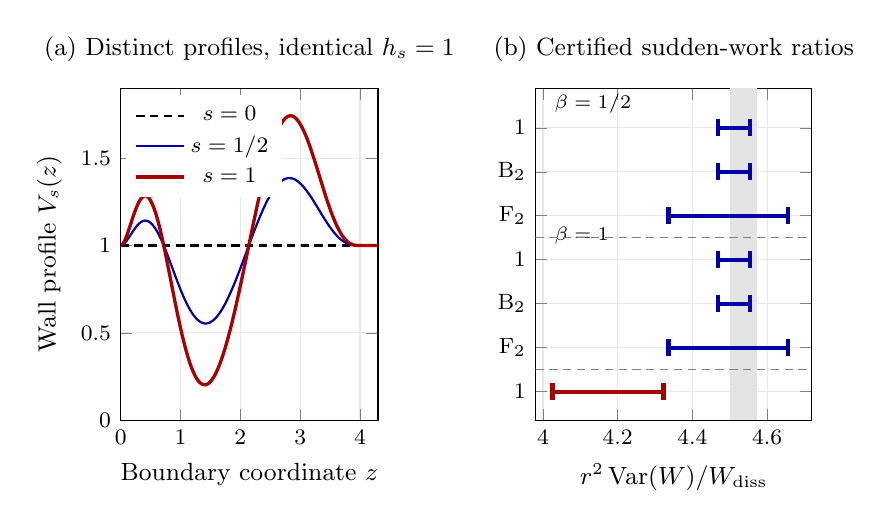
\begin{tikzpicture}
\begin{axis}[
 name=profiles,width=0.40\textwidth,height=5.8cm,
 xmin=0,xmax=4.3,ymin=0,ymax=1.9,
 xlabel={Boundary coordinate $z$},ylabel={Wall profile $V_s(z)$},
 title={(a) Distinct profiles, identical $h_s=1$},
 title style={font=\small},label style={font=\small},
 tick label style={font=\footnotesize},grid=major,
 grid style={gray!18},legend style={font=\footnotesize,draw=none,at={(0.02,0.98)},anchor=north west},
 domain=0:4.3,samples=181]
\addplot[black,densely dashed,thick]{1};
\addlegendentry{$s=0$}
\addplot[blue!65!black,thick]
 {1+0.3*(12*x^2*max(0,1-x/4)^5-10*x^3*max(0,1-x/4)^4+1.25*x^4*max(0,1-x/4)^3-8*x^3*max(0,1-x/4)^5+2.5*x^4*max(0,1-x/4)^4)/(1+0.3*x^4*max(0,1-x/4)^5)};
\addlegendentry{$s=1/2$}
\addplot[red!65!black,very thick]
 {1+0.6*(12*x^2*max(0,1-x/4)^5-10*x^3*max(0,1-x/4)^4+1.25*x^4*max(0,1-x/4)^3-8*x^3*max(0,1-x/4)^5+2.5*x^4*max(0,1-x/4)^4)/(1+0.6*x^4*max(0,1-x/4)^5)};
\addlegendentry{$s=1$}
\end{axis}
\begin{axis}[
 at={(profiles.east)},anchor=west,xshift=2.0cm,
 width=0.42\textwidth,height=5.8cm,
 xmin=3.98,xmax=4.72,ymin=-0.65,ymax=6.9,
 xlabel={$r^2\operatorname{Var}(W)/W_{\mathrm{diss}}$},
 title={(b) Certified sudden-work ratios},
 title style={font=\small},label style={font=\small},
 tick label style={font=\footnotesize},
 ytick={0,1,2,3,4,5,6},
 yticklabels={$1$, $\mathrm{F}_2$, $\mathrm{B}_2$, $1$, $\mathrm{F}_2$, $\mathrm{B}_2$, $1$},
 xtick={4.0,4.2,4.4,4.6},grid=major,grid style={gray!18}]
\path[fill=gray!22,draw=none] (axis cs:4.49973,-0.65) rectangle (axis cs:4.57308,6.9);
\addplot[red!65!black,line width=1.6pt,mark=|,mark size=3pt]
 coordinates {(4.02532,0) (4.32246,0)};
\addplot[blue!65!black,line width=1.6pt,mark=|,mark size=3pt]
 coordinates {(4.33631,1) (4.65600,1)};
\addplot[blue!65!black,line width=1.6pt,mark=|,mark size=3pt]
 coordinates {(4.46796,2) (4.55425,2)};
\addplot[blue!65!black,line width=1.6pt,mark=|,mark size=3pt]
 coordinates {(4.46796,3) (4.55425,3)};
\addplot[blue!65!black,line width=1.6pt,mark=|,mark size=3pt]
 coordinates {(4.33628,4) (4.65605,4)};
\addplot[blue!65!black,line width=1.6pt,mark=|,mark size=3pt]
 coordinates {(4.46796,5) (4.55425,5)};
\addplot[blue!65!black,line width=1.6pt,mark=|,mark size=3pt]
 coordinates {(4.46796,6) (4.55425,6)};
\node[font=\scriptsize,anchor=west] at (axis cs:4.005,6.55) {$\beta=1/2$};
\node[font=\scriptsize,anchor=west] at (axis cs:4.005,3.55) {$\beta=1$};
\draw[gray,densely dashed] (axis cs:3.98,0.5)--(axis cs:4.72,0.5);
\draw[gray,densely dashed] (axis cs:3.98,3.5)--(axis cs:4.72,3.5);
\end{axis}
\end{tikzpicture}
\caption{A calibrated profile change and its finite-wall consequence. (a) The exact profiles of Eq.~\eqref{eq:profile}; curves are evaluations of that formula, not a numerical calibration fit. (b) Horizontal segments are deterministic outward enclosures, not statistical error bars. The six blue intervals use $r=0.025$; $1$, $\mathrm B_2$, and $\mathrm F_2$ denote one particle and canonical two-boson and two-fermion preparations. The bottom red interval uses one particle, $r=0.1$, and $\beta=1$. The gray band encloses the common asymptotic profile quotient. Its disjointness from the red interval demonstrates why a finite-wall prediction needs an independent error certificate. No midpoint is used as an estimated exact value. Plotting code renders the stated formulas and certificate intervals; it does not generate or infer the data.}
\label{fig:profile-ratios}
\end{figure*}

At $r=0.025$, the same endpoint profiles permit a certified comparison at $\beta=0.5$ and $1$, for one particle and canonical $N=2$ Bose and Fermi preparations (Fig.~\ref{fig:profile-ratios}). Full thermal-tail and exchange bounds enclose all six sudden ratios in
\begin{equation}
 4.33628569<\frac{r^2\Var W}{\Wd}<4.65604645.\label{eq:preparations}
\end{equation}
Their relative deviation from the enclosed limiting profile quotient is at most $5.178\%$. Bose and Fermi variances differ by more than a factor $2.5$ in this comparison; the normalized agreement is not an assertion that their fluctuation magnitudes coincide. Both chosen temperatures are low, and the certificate does not establish broad temperature-independent finite-wall behavior.

A limited design question can also be answered without a global optimization claim. Return to the one-particle baseline $r=0.1$, $\beta=1$. Replace the amplitude $0.6$ in Eq.~\eqref{eq:profile} by one of $\{0.3,0.4,0.5,0.55,0.6,0.625,0.64,0.65\}$. Keep the same initial state, collar, duration $\tau=0.001$, calibration, bounds $0.15<V_s<2$, and reporting contract. Every candidate also satisfies $\sup_s\norm{\partial_sH_s}<110$. Evaluating the same rigorous lower guarantee for all eight gives the largest lower endpoint at amplitude $0.65$:
\begin{equation}
 \Prob(A)>2.12665098\times10^{-5},\qquad N_{95}=140865.
 \label{eq:design}
\end{equation}
This reduces the sufficient budget by $13.50865\%$ relative to the baseline. The true-probability intervals overlap, so no actual-probability ranking or continuous/global optimum follows. Work-statistics control is an established subject \cite{Solon,Miller}; the calculation here optimizes a particular certified detector guarantee over a declared finite family.

For independent Bernoulli trials with $p_A\ge p_L>0$, the exact sufficient detection budget is $\lceil\log(0.05)/\log(1-p_L)\rceil$. For estimating the frequency to $10\%$ relative error with $95\%$ confidence, a distribution-free Chebyshev bound instead gives the sufficient count $\lceil2000/p_L\rceil$. For the baseline at $\tau=0.001$, the latter is $108732970$. These integer counts use the more precise lower endpoints in Appendix~\ref{app:numerical}, not the shorter summaries in Table~\ref{tab:duration}. Detecting an event is therefore not the same operational task as measuring its probability precisely.

Moment estimation is more demanding still. For the smooth sudden switch, the potential difference belongs to $W^{2,\infty}$, which gives a finite fourth TPM moment. A separately specified full-range fine-energy reporting model yields a sufficient budget of $3828614895$ preparations for the stated ratio estimator to lie in $[3.59919694,4.82438415]$ with probability at least $95\%$. This is an a priori estimator guarantee, not a confidence interval centered on observed data. This conservative upper budget is not a lower bound on all estimators. It does not apply to the coarse detector in Eq.~\eqref{eq:detector}, and no finite-time fourth-moment or ratio-estimation statement is inferred from it.

\section{Discussion}

The missing information in a calibrated wall is not another equilibrium eigenvalue correction. It is the response of the microscopic state to a physical change of profile. In one dimension, that response is a square-integrable disturbance whose full outgoing spectral measure determines probability and energetic cost. The finite-order calibration leaves nonzero tangent directions, and microscopic-time driving resolves them. In smooth cavities, the leading sudden response separates into a known pressure factor and a positive profile energy; canonical ideal statistics changes the pressure without removing the microscopic distinction.

This is consistent with effective descriptions. Matching a low-energy stationary response does not also match a high-frequency intervention or its control operator. The asymptotic drive has duration $\eta r^2$ and the finite example specifies its wall scale, temperature and detector assumptions. Neither supplies a fixed-bandwidth experiment as $r\downarrow0$. The growing work variance is not itself evidence of an attainable metrological advantage, and the certified resource budgets prevent that interpretation.

The results leave several separate extensions: interacting particles, growing particle number, finite-time dynamics in arbitrary curved cavities, uniform calibration-order estimates, and a material-specific implementation of the reporting contract. None is needed for the complete results established here. The operational conclusion is narrower and precise: the stated stationary calibration, even when preserved throughout the drive, is insufficient to determine microscopic work, and the resulting difference can be followed from the actual Hamiltonian to a bounded-energy finite-parameter observation.


\paragraph*{Note on AI Use}
The author declares the substantial use of consumer-grade Gemini-3 and GPT-6 models for literature search, exploring and developing ideas, codes and proofs, drafting and LaTeX typesetting; the author takes full and sole responsibility for all contents of this work.

\paragraph*{Data availability.}
Repository - 
\href{https://github.com/arun-chandru/calibrated_work}{github.com/arun-chandru/calibrated\_work}

\newpage

\appendix
\section{Stationary calibration and complete thermal control on the interval}
\label{app:intervalcalibration}

We derive the interval estimates needed for the complete transition law. The
spectral label starts at $n=1$. Unless a parameter is displayed, the wall
profile, exterior length $b$, inverse temperature $\beta$, and any finite
calibration order are fixed before $r$ tends to zero. Constants can depend on
these data. For a compact path with a common positive constant tail, the
constants below are uniform along the path.

\subsection{The finite exterior endpoint and the low-energy roots}

Choose a distance $\ell$ beyond which $V=v_\infty>0$. For complex scaled
energy $\epsilon$ near zero, solve the wall equation on $[0,\ell]$ with the
exact decaying tail and normalize its solution by
$w_{V,\epsilon}(0)=1$. The normalization is nonzero at zero energy and
remains so in a sufficiently small complex disk. Finite-interval ODE
dependence and the analytic branch
$\gamma(\epsilon)=\sqrt{v_\infty-\epsilon}$, with positive real part,
therefore make
\begin{equation}
 h_V(\epsilon)=-w_{V,\epsilon}'(0)
 \label{eq:coreweyl}
\end{equation}
analytic on that disk. On a smaller real interval it is bounded below by
$h_V/2$. A compact family of the profiles considered here admits one such
disk: the ODE transfer matrices depend continuously on the family and the
positive normalized zero-energy solutions have no zeros.

The actual scaled exterior has length $b/r$. Write
$w_{V,r,\epsilon}(0)=1$ for its wall solution that vanishes at $b/r$, and
$h_{V,r}(\epsilon)=-w_{V,r,\epsilon}'(0)$. Its exact logarithmic derivative
at $\ell$, for sufficiently small $r$, is
\begin{equation}
 -\frac{w_{V,r,\epsilon}'(\ell)}{w_{V,r,\epsilon}(\ell)}
 =\gamma(\epsilon)
       \coth\!\left[\gamma(\epsilon)(b/r-\ell)\right].
 \label{eq:corecoth}
\end{equation}
Transport through $[0,\ell]$ is analytic in this datum. It follows that
$h_{V,r}-h_V=O(e^{-c/r})$ uniformly on a smaller disk. Any fixed finite
number of energy derivatives obeys the same estimate after decreasing
$c$. Derivatives of the hyperbolic function produce only polynomial
factors in $1/r$, which the exponential absorbs. The same construction
shows, after extending the finite wall solution by zero beyond $b/r$,
\begin{equation}
 \begin{gathered}
 \norm{w_{V,r,\epsilon}-w_V}_{L^2(0,\infty)}
 \le C|\epsilon|+Ce^{-c/r},\\
 \norm{w_{V,r,\epsilon}}_{L^2(0,b/r)}\le C.
 \end{gathered}
 \label{eq:corewallnorm}
\end{equation}
These bounds also hold with a sufficiently small fixed positive exponential
weight in $z$ and with the energy derivatives that are used below. They
follow directly from the two exponential tail components: the component
reflected by the distant Dirichlet endpoint is exponentially small, as is
the omitted infinite tail. Thus the finite outer wall has not been
replaced by a half-line without an error estimate.

All eigenvalues of the finite one-dimensional Dirichlet problem are simple.
Min--max gives, for every spectral index,
\begin{equation}
 \frac{\pi^2n^2}{(1+b)^2}\le e_{V,n}(r)\le\lambda_n,
 \qquad \lambda_n=(n\pi)^2.
 \label{eq:coreglobalbounds}
\end{equation}
For the upper bound one uses interior Dirichlet orbitals, extended by zero,
as quadratic-form trial functions. If $e=k^2$ and $r^2e$ is in the selected
small real interval, continuity of the value and derivative at $y=1$
gives the exact root equation
\begin{equation}
 k+\arctan\frac{rk}{h_{V,r}(r^2k^2)}=n\pi.
 \label{eq:coreroot}
\end{equation}
There are no wall-Weyl poles in this interval. Green's identity gives
\begin{equation}
 \partial_\epsilon h_{V,r}(\epsilon)
       =-\int_0^{b/r}w_{V,r,\epsilon}(z)^2\,\dd z<0,
 \label{eq:coreweylderivative}
\end{equation}
so the left side of Eq.~\eqref{eq:coreroot} is strictly increasing in $k$
there. Its roots have the ordered labels shown in that equation.

Let
\begin{equation}
 K_r=\lfloor c r^{-1/3}\rfloor
 \label{eq:corethermalcutoff}
\end{equation}
with a fixed sufficiently small $c>0$. Equations~\eqref{eq:coreglobalbounds}
and \eqref{eq:coreroot} apply uniformly to the first $K_r+1$ roots when
$r$ is small. In particular,
\begin{equation}
 e_{V,n}(r)=\frac{\lambda_n}{(1+r/h_V)^2}
            +O\!\left(r^3(\lambda_n+\lambda_n^2)\right),
 \qquad n\le K_r.
 \label{eq:corerootexpansion}
\end{equation}
The uniform remainder can be seen without extrapolating a fixed-index
expansion. First omit the exponentially small finite-endpoint correction,
put $k=n\pi v$ and $q=rn\pi$, and rewrite the root equation as
\begin{equation}
 v+r\frac{v}{h_V(q^2v^2)}
       \frac{\arctan[qv/h_V(q^2v^2)]}{qv/h_V(q^2v^2)}=1.
 \label{eq:coreanalyticroot}
\end{equation}
The quotient has its continuous analytic value at zero. The equation is
analytic in $(r,q^2,v)$ and its $v$ derivative is nonzero near $(0,0,1)$.
At $q=0$ the solution is $(1+r/h_V)^{-1}$; at $r=0$ it is one for every
small $q$. Its difference from $(1+r/h_V)^{-1}$ consequently has the
factor $rq^2$ and a bounded analytic coefficient. Squaring $k$ proves
Eq.~\eqref{eq:corerootexpansion}. Reintroducing
Eq.~\eqref{eq:corecoth} adds only an exponentially small term, uniformly
on this index range.

For two profiles satisfying
$h_1^{(j)}(0)=h_0^{(j)}(0)$, $0\le j\le J$, analyticity implies
$h_1(\epsilon)-h_0(\epsilon)=O(\epsilon^{J+1})$. Their two root
functions in Eq.~\eqref{eq:coreroot} differ by at most
$Crk|r^2k^2|^{J+1}+Ce^{-c/r}$ on the low-root range. Their derivatives
are bounded below. Comparing their zeros and then their squares gives
\begin{equation}
 |e_{1,n}(r)-e_{0,n}(r)|
       \le C_Jr^{2J+3}P_J(n),\qquad n\le K_r,
 \label{eq:corematchedroots}
\end{equation}
where $P_J$ is a fixed polynomial. Exponential endpoint errors are absorbed
in the right side. The same estimate is uniform between the initial
profile and every member of a compact exactly calibrated path. The
polynomial degree and constants can depend on $J$; no limit with growing
$J$ is taken.

\subsection{Normalization and the surviving wall disturbance}

Choose real eigenfunctions with positive interior normalization coefficient.
The exact normalized low orbital is
\begin{equation}
 \phi_{V,n}(y)=
 \begin{cases}
 a_{V,n}\sin(k_{V,n}y),&0<y<1,\\
  \begin{aligned} &a_{V,n}\sin k_{V,n}\,\\[-2pt]
  &\times w_{V,r,r^2e_{V,n}}((y-1)/r),\end{aligned}&1<y<1+b,
 \end{cases}
 \label{eq:coreorbital}
\end{equation}
where
\begin{align}
 a_{V,n}^{-2}
 &=\frac12-\frac{\sin(2k_{V,n})}{4k_{V,n}}\nonumber\\
 &\quad+r\sin^2 k_{V,n}
            \int_0^{b/r}w_{V,r,r^2e_{V,n}}^2\,\dd z.
 \label{eq:corenormalization}
\end{align}
The matching condition also gives
\begin{equation}
 \sin^2 k_{V,n}
     =\frac{r^2e_{V,n}}
             {h_{V,r}(r^2e_{V,n})^2+r^2e_{V,n}}.
 \label{eq:coreamplitudeidentity}
\end{equation}
Equations~\eqref{eq:corewallnorm}--\eqref{eq:coreamplitudeidentity} imply
$a_{V,n}^2=2+O(r)$ and
\begin{equation}
 \norm{\mathbf1_{y>1}\phi_{V,n}}\le Cnr^{3/2},
 \qquad n\le K_r.
 \label{eq:corewallpopulation}
\end{equation}
For each fixed $n$ and a profile of response $h$,
\begin{equation}
 \frac{a_{V,n}\sin k_{V,n}}r\longrightarrow
 c_n=\frac{(-1)^{n+1}\sqrt{2\lambda_n}}h.
 \label{eq:coreamplitudelimit}
\end{equation}

For endpoints of equal $h$, Eq.~\eqref{eq:corematchedroots} with $J=0$
gives an $O(r^3P(n))$ phase difference. In
Eq.~\eqref{eq:corenormalization}, the difference of the interior terms is
of this order. Each wall term is itself $O(r^3n^2)$, so the difference of
the normalization coefficients is also $O(r^3P(n))$. The interior
orbital difference is therefore $O(r^3P(n))$ in $L^2(0,1)$.

Introduce the unitary scaling to the interval
$I_r=(-1/r,b/r)$,
\begin{equation}
 (S_r\phi)(z)=\sqrt r\,\phi(1+rz),\qquad
 \psi_{j,n,r}=S_r\phi_{j,n},
 \label{eq:corescaling}
\end{equation}
and extend its vectors by zero to $\R$. With $u=w_0-w_1$ and
$\widehat w_0=\mathbf1_{z>0}w_0$, the preceding estimates give
\begin{align}
 r^{-3/2}(\psi_{0,n,r}-\psi_{1,n,r})&\longrightarrow c_nu,
       \label{eq:corestaticdisturbance}\\
 r^{-3/2}\mathbf1_{z>0}\psi_{0,n,r}&\longrightarrow
           c_n\widehat w_0
       \label{eq:corestaticsource}
\end{align}
strongly in $L^2(\R)$ for each fixed $n$. On the negative half-line the
norm in Eq.~\eqref{eq:corestaticdisturbance} is
$O(r^{3/2}P(n))$ and vanishes. On the positive half-line,
Eqs.~\eqref{eq:corewallnorm} and \eqref{eq:coreamplitudelimit} identify
the entire surviving norm, including the exponentially decaying tail.
The same estimates also supply the uniform bound
\begin{equation}
 \norm{\phi_{0,n}-\phi_{1,n}}\le Cr^{3/2}P(n),
 \qquad n\le K_r.
 \label{eq:coreorbitaldifferencebound}
\end{equation}

\subsection{The complete Gibbs sum}

Writing $p_{n,r}=e^{-\beta e_{0,n}}/Z_{0,r}$, the global eigenvalue bounds
give
\begin{equation}
 p_{n,r}\le e^{\beta\pi^2}
       e^{-\beta\pi^2n^2/(1+b)^2}.
 \label{eq:coregibbsmajorant}
\end{equation}
Indeed $Z_{0,r}\ge e^{-\beta e_{0,1}}\ge e^{-\beta\pi^2}$.
Thus every fixed polynomial in the initial label is summable uniformly in
small $r$. At each fixed label $e_{0,n}\to\lambda_n$; dominated
convergence yields $Z_{0,r}\to Z_D$ and $p_{n,r}\to p_n^D$, where
$p_n^D=e^{-\beta\lambda_n}/Z_D$. In particular,
\begin{equation}
 \sum_{n\ge1}p_n^Dc_n^2=\frac{2U_D(\beta)}{h^2}=C_\beta.
 \label{eq:corethermalcoefficient}
\end{equation}

For the calibrated partition-function difference, the exponential
mean-value inequality and Eq.~\eqref{eq:corematchedroots} bound the low
sum by
\begin{equation}
 \sum_{n\le K_r}
 |e^{-\beta e_{1,n}}-e^{-\beta e_{0,n}}|
 \le Cr^{2J+3}\sum_{n\ge1}P_J(n)e^{-c_0n^2}.
 \label{eq:corelowpartition}
\end{equation}
The two complementary sums obey
\begin{equation}
 \sum_{n>K_r}e^{-\beta e_{j,n}}
     \le Ce^{-c_1r^{-2/3}},\qquad j=0,1.
 \label{eq:corehightail}
\end{equation}
Since both partition functions have a fixed positive lower bound, it
follows that
\begin{equation}
 |\log Z_{1,r}-\log Z_{0,r}|=O(r^{2J+3}).
 \label{eq:corematchedpartition}
\end{equation}
The same argument is uniform along the compact path. It proves the
full thermal calibration statement, including initially populated
above-barrier and exterior states. No differentiated heat-trace expansion
is needed for this comparison or for the dynamic moments below.

\section{The complete finite-time transition measure and its moments}
\label{app:corefinitework}

Fix $0<\eta<\infty$. In this appendix $s\mapsto V_s$ is a
$C^1([0,1];L^\infty(0,\infty))$ path of positive profiles with uniformly
bounded spatial $C^2$ norms. There are a common finite $\ell$ and a common
$v_\infty>0$ such that $V_s(z)=v_\infty$ for $z\ge\ell$.
Only the endpoint matching $h_0=h_1=h$ is needed until the calibrated
construction in Appendix~\ref{app:corejets}. The physical duration is
$\eta r^2$ and the full path is fixed before the wall limit.

The scaled operators and their propagators are
\begin{equation}
 \begin{gathered}
 A_{s,r}=r^2S_rH_{s,r}S_r^{-1}
          =-\partial_z^2+V_{s,+}(z)\quad\hbox{on }I_r,\\
 i\partial_sU_r(s,t)=\eta A_{s,r}U_r(s,t).
 \end{gathered}
 \label{eq:coreintervaldynamics}
\end{equation}
The rescaled physical propagator is $U_r(1,0)$. The limiting operators
$A_s=-\partial_z^2+V_{s,+}$ act on $L^2(\R)$ with the common domain
$H^2(\R)$. For equal endpoint response, the zero extension of
$u=w_0-w_1$ has both zero value and zero derivative at the interface.
Consequently
\begin{equation}
 u\in H^2(\R),\qquad A_1u=(V_1-V_0)_+\widehat w_0.
 \label{eq:coreinterfacecancellation}
\end{equation}
There is no singular interface source in this identity.

\subsection{Convergence of the actual outgoing disturbance}

The expanding-interval Dirichlet quadratic forms converge to the
full-line form: compactly supported smooth functions eventually lie in
every interval, the forms agree on them, and weak lower semicontinuity
gives the reverse inequality. Thus the resolvents converge strongly.
One can use ordinary full-Hilbert-space strong-resolvent convergence by
adjoining a zero operator on $L^2(I_r^c)$; its exterior projection tends
strongly to zero. The autonomous propagators then converge strongly,
uniformly on compact time intervals. Expand the time-dependent
propagators about $A_{0,r}$ using the bounded perturbation
$(V_s-V_0)_+$ restricted to $I_r$. Every finite Dyson term converges by dominated integration,
and the remaining series has a common factorial bound. Therefore
\begin{equation}
 U_r(s,t)v_r\longrightarrow U(s,t)v
 \quad\hbox{uniformly for }0\le t\le s\le1
 \label{eq:corepropagatorlimit}
\end{equation}
whenever $v_r\to v$ strongly. Operator-norm convergence of the
expanding-domain propagators is not being used.

Set $\epsilon_{j,n,r}=r^2e_{j,n}$ and
$\alpha_{n,r}=e^{-i\eta\epsilon_{0,n,r}}$. Exact Duhamel expansion about
the initial eigenphase gives
\begin{align}
 U_r(s,0)\psi_{0,n,r}
 &=e^{-i\eta s\epsilon_{0,n,r}}\psi_{0,n,r}
          +r^{3/2}q_{n,r}(s),\label{eq:coreduhamel}\\
 q_{n,r}(s)
 &=-i\eta\int_0^sU_r(s,t)(V_t-V_0)_+\nonumber\\
 &\qquad\times e^{-i\eta t\epsilon_{0,n,r}}
         r^{-3/2}\psi_{0,n,r}\,\dd t.
 \label{eq:coreduhamelsource}
\end{align}
Only the localized input to the integral must converge. By
Eqs.~\eqref{eq:corestaticsource} and \eqref{eq:corepropagatorlimit},
$q_{n,r}(s)\to c_nq_s$ strongly and uniformly in $s$, with $q_s$ as in
Eq.~\eqref{eq:q}. Combining this limit with
Eq.~\eqref{eq:corestaticdisturbance} proves
\begin{equation}
 \begin{gathered}
 \mathcal D_{n,r}:=r^{-3/2}
 [U_r(1,0)\psi_{0,n,r}-\alpha_{n,r}\psi_{1,n,r}]\\
       \longrightarrow c_nd,\qquad d=u+q_1,
 \end{gathered}
 \label{eq:coreoutgoinglimit}
\end{equation}
strongly on the full line. The larger interior orbital change that would
arise from unequal $h$ has canceled before this limit is taken.

\subsection{An independent energy-source limit}

At every finite $r$ the bounded time-dependent potentials have a common
operator domain. Differentiating
$U_r(1,s)A_{s,r}U_r(s,0)$ on that domain gives
\begin{align}
 A_{1,r}U_r(1,0)-U_r(1,0)A_{0,r}
  =\int_0^1U_r(1,s)\dot V_{s,+}U_r(s,0)\,\dd s.
 \label{eq:coreenergydefect}
\end{align}
The Hamiltonian terms in the derivative cancel; no factor $\eta$
multiplies the right side. This expression extends to a bounded operator
with norm at most
\begin{equation}
 \mathsf T=\int_0^1\norm{\dot V_s}_\infty\,\dd s.
 \label{eq:corevariationbudget}
\end{equation}
The identity also follows by approximation with smooth time coefficients,
so its use does not require extra time derivatives of the potential.

Apply Eq.~\eqref{eq:coreenergydefect} to the initial eigenvector, divide
by $r^{3/2}$ and use Eq.~\eqref{eq:coreduhamel}. The resulting source
satisfies
\begin{align}
 \mathcal G_{n,r}
 &:=r^{-3/2}(A_{1,r}-\epsilon_{0,n,r})
                    U_r(1,0)\psi_{0,n,r}\nonumber\\
 &\longrightarrow c_n\int_0^1U(1,s)\dot V_{s,+}
                         (\widehat w_0+q_s)\,\dd s=c_ng
 \label{eq:coreenergysourcelimit}
\end{align}
strongly. The factor $\dot V_{s,+}$ vanishes on the left, so no derivative
acts on the discontinuous zero extension $\widehat w_0$.

For $B_{n,r}=A_{1,r}-\epsilon_{0,n,r}$, subtracting the reference
eigenvector in Eq.~\eqref{eq:coreoutgoinglimit} gives
\begin{align}
 B_{n,r}\mathcal D_{n,r}
 &=\mathcal G_{n,r}
 -\alpha_{n,r}r^{-3/2}(\epsilon_{1,n,r}-\epsilon_{0,n,r})
                         \psi_{1,n,r}\nonumber\\
 &\longrightarrow c_ng.
 \label{eq:coregraphlimit}
\end{align}
The subtracted vector has norm $O(r^{7/2}P(n))$ at fixed $n$, by
Eq.~\eqref{eq:corematchedroots} with $J=0$. Also
$\epsilon_{0,n,r}\mathcal D_{n,r}\to0$. Apply
$(A_{1,r}+i)^{-1}$ to
$A_{1,r}\mathcal D_{n,r}+i\mathcal D_{n,r}$ and pass to the strong limit.
Equations~\eqref{eq:coreoutgoinglimit} and \eqref{eq:coregraphlimit}
then establish
\begin{equation}
 d\in D(A_1),\qquad A_1d=g.
 \label{eq:coregraphidentity}
\end{equation}
This argument obtains the limiting domain from graph convergence. It
does not differentiate an unverified limiting vector.

\subsection{The exact off-label measure and its weighted totals}

Let $P_{n,r}$ be the rank-one projection onto the final orbital
$\psi_{1,n,r}$. For fixed $n$, this orbital converges weakly to zero in
$L^2(\R)$. Its norm is one, whereas Eq.~\eqref{eq:coreorbital} shows
that its norm on each fixed compact interval in $z$ tends to zero;
compactly supported test functions are dense. Hence its projection of a
strongly convergent vector tends to zero. Since $P_{n,r}$ commutes with
$B_{n,r}$, Eqs.~\eqref{eq:coreoutgoinglimit} and
\eqref{eq:coregraphlimit} give
\begin{equation}
 Y_{n,r}=(1-P_{n,r})\mathcal D_{n,r}\to c_nd,
 \qquad B_{n,r}Y_{n,r}\to c_nA_1d
 \label{eq:coreprojectedgraph}
\end{equation}
strongly.

The rescaled conditional off-label measure is exactly
\begin{align}
 \nu_{n,r}(S)
 &=r^{-3}\sum_{m\ne n}
   |\langle\psi_{1,m,r},U_r(1,0)\psi_{0,n,r}\rangle|^2\nonumber\\
 &\qquad\times\mathbf1_S(\epsilon_{1,m,r}-\epsilon_{0,n,r})\nonumber\\
 &=\langle Y_{n,r},\mathbf1_S(B_{n,r})Y_{n,r}\rangle.
 \label{eq:coreexactmeasure}
\end{align}
Subtracting the reference eigenvector changes no amplitude with $m\ne n$.
Strong functional calculus and Eq.~\eqref{eq:coreprojectedgraph} prove
weak convergence against continuous compactly supported tests, together
with the total-mass limit,
\begin{equation}
 \nu_{n,r}\Longrightarrow c_n^2\mu_d^{A_1},\qquad
 \nu_{n,r}(\R)\to c_n^2\norm d^2.
 \label{eq:corefixedlabelmeasure}
\end{equation}
No division by a possibly small work gap occurs.

The spectral measure of $B_{n,r}Y_{n,r}$ is
$E^2\dd\nu_{n,r}(E)$. Its strong vector limit in
Eq.~\eqref{eq:coreprojectedgraph} independently gives the weak limit and
the full second-energy-weighted total. The first total follows from the
convergent inner product. Explicitly,
\begin{align}
 \int\dd\nu_{n,r}&=\norm{Y_{n,r}}^2\to c_n^2\norm d^2,\nonumber\\
 \int E\,\dd\nu_{n,r}
 &=\langle Y_{n,r},B_{n,r}Y_{n,r}\rangle
       \to c_n^2\langle d,A_1d\rangle,\nonumber\\
 \int E^2\,\dd\nu_{n,r}
 &=\norm{B_{n,r}Y_{n,r}}^2\to c_n^2\norm{A_1d}^2.
 \label{eq:corefixedlabelmoments}
\end{align}
The first moment can also be passed by truncation: for any positive
measure with these finite totals,
\begin{equation}
 \begin{gathered}
 \int_{|E|>M}|E|\,\dd\nu\le M^{-1}\int E^2\,\dd\nu,
 \\
 \int_{|E|<a}|E|\,\dd\nu\le a\int\dd\nu.
 \end{gathered}
 \label{eq:corefirstmomenttails}
\end{equation}
Thus the unweighted convergence is not being used alone to infer
unbounded work moments.

\subsection{Summing the full preparation and recovering physical work}

The fixed-label limits admit a uniform thermal majorant. Put
\begin{equation}
 \mathsf B=\int_0^1\norm{V_s-V_0}_\infty\,\dd s,
 \qquad Q=\mathbf1_{z>0}.
 \label{eq:corepathbudget}
\end{equation}
Unitarity in Eq.~\eqref{eq:coreduhamel} gives, for every initial
eigenstate,
\begin{align}
 \sup_s\norm{QU_r(s,0)\psi_{0,n,r}}
     &\le(1+\eta\mathsf B)\norm{Q\psi_{0,n,r}},\nonumber\\
 \norm{\mathcal G_{n,r}}
     &\le r^{-3/2}\mathsf T(1+\eta\mathsf B)
                              \norm{Q\psi_{0,n,r}}.
 \label{eq:coreuniformsources}
\end{align}
For $n\le K_r$, Eqs.~\eqref{eq:corewallpopulation},
\eqref{eq:coreorbitaldifferencebound}, and
\eqref{eq:coreuniformsources} bound $\mathcal D_{n,r}$ and
$\mathcal G_{n,r}$, and hence the three quantities in
Eq.~\eqref{eq:corefixedlabelmoments}, by fixed polynomials in $n$.
Their thermal sums are dominated by Eq.~\eqref{eq:coregibbsmajorant}.

For $n>K_r$, no low-energy orbital approximation is used. A row's
off-label probability is at most one, and
Eq.~\eqref{eq:coreenergydefect} applied to its normalized initial
eigenvector gives
\begin{equation}
 \sum_m(\epsilon_{1,m,r}-\epsilon_{0,n,r})^2
 |\langle\psi_{1,m,r},U_r\psi_{0,n,r}\rangle|^2
       \le\mathsf T^2.
 \label{eq:coreallindexenergy}
\end{equation}
Consequently the high initial-label contribution to the scaled total
probability and scaled second moment is bounded by
\begin{equation}
 Cr^{-3}\sum_{n>K_r}p_{n,r}
       \le Cr^{-3}e^{-c_1r^{-2/3}}\longrightarrow0.
 \label{eq:corehighdynamicstail}
\end{equation}
Cauchy--Schwarz within each row bounds its absolute scaled first moment
by $r^{-3}\mathsf T$, so the same thermal estimate applies to that
moment. This controls every initial label and the complete final
spectrum.

Let
$\nu_r(S)=r^{-3}\Prob(r^2W\in S,m\ne n)=\sum_np_{n,r}\nu_{n,r}(S)$.
The low-label polynomial majorant, high-label estimate, and
Eq.~\eqref{eq:corethermalcoefficient} now yield
\begin{align}
 \nu_r&\Longrightarrow C_\beta\mu_d^{A_1},\nonumber\\
 E^2\dd\nu_r(E)&\Longrightarrow C_\beta\dd\mu_{A_1d}^{A_1}(E),
 \label{eq:corefullmeasure}
\end{align}
including both total masses. Their first totals converge as in
Eq.~\eqref{eq:corefixedlabelmoments}. The first-weighted measures have
the same passage by Eq.~\eqref{eq:corefirstmomenttails}.

For the omitted same-label sector,
$|e_{1,n}-e_{0,n}|\le Cr^3P(n)$ on the low range. Its thermal mean is
therefore $O(r^3)$, and its contribution to $r\E W^2$ is $O(r^7)$.
For the high range the full row bound
Eq.~\eqref{eq:corehighdynamicstail} already applies. Since
\begin{equation}
 \begin{gathered}
 \int E\,\dd\nu_r
       =r^{-1}\E[W\mathbf1_{m\ne n}],\\
 \int E^2\,\dd\nu_r
        =r\E[W^2\mathbf1_{m\ne n}],
 \end{gathered}
 \label{eq:corephysicalmoments}
\end{equation}
we obtain $\E W=O(r)$. Hence $r(\E W)^2\to0$. Equation
\eqref{eq:corematchedpartition} gives $\Delta F_r=O(r^3)$ and finally
\begin{align}
 r^{-3}\Prob(m\ne n)&\longrightarrow C_\beta\norm d^2,\nonumber\\
 \frac{\Wd}{r}&\longrightarrow C_\beta\langle d,A_1d\rangle,\nonumber\\
 r\Var W&\longrightarrow C_\beta\norm{A_1d}^2.
 \label{eq:corefullmoments}
\end{align}
The first line describes a change of ordered label. The same-label work
need not vanish, even though its contribution to the displayed moment
scales does.

The full-line operator $A_1$ is nonnegative and has no eigenvalues. At
positive energy an $L^2$ solution on the free negative half-line must
vanish there; at zero energy the same follows for an affine solution.
ODE uniqueness then makes the solution zero everywhere, while
nonnegativity excludes negative eigenvalues. Its scalar spectral
measures are consequently atomless and assign full mass to
$(0,\infty)$. Together with the independently proved total masses in
Eq.~\eqref{eq:corefullmeasure}, this excludes loss of probability or
second-moment weight at zero or either infinity. Atomlessness also
gives uniform convergence of cumulative measures, by a finite-grid
argument on a large compact interval and small tails outside it.
Negative work was retained throughout in $B_{n,r}$; it was not removed
by an assumed sign. Conditional on $m\ne n$, the limiting scaled-work
law is $\mu_d^{A_1}/\norm d^2$ when $d\ne0$. Since $\ker A_1=0$, all
three coefficients in Eq.~\eqref{eq:corefullmoments} are strictly
positive in that case.

For a sudden change the argument simplifies to $U_r=I$, $q_s=0$,
$d=u$, and $g=f$. The endpoint stationary estimates and
$A_1u=f$ supply the same graph limits directly, so this case does not
require a common-tail driving interpolation. The high-label bound uses
the bounded defect $A_{1,r}-A_{0,r}=(V_1-V_0)_+$, with
$\norm{V_1-V_0}_\infty$ in place of $\mathsf T$ in
Eq.~\eqref{eq:coreallindexenergy}. It proves
Eqs.~\eqref{eq:suddenlaw}, \eqref{eq:suddenprob},
\eqref{eq:suddenmean}, and \eqref{eq:suddenvar}. Equivalently, the
spectral theorem gives the finite identities
\begin{equation}
 \begin{gathered}
 \int E^{-2}\dd\mu_f=\norm u^2,\\
 \int E^{-1}\dd\mu_f=\calE_1(u),\\
 \int\dd\mu_f=\norm f^2.
 \end{gathered}
 \label{eq:coresuddenspectralmoments}
\end{equation}
Their first pairing is consistent with the elementary energy
cancellation
$\int(V_1-V_0)w_0^2=\calE_1(u)$: the trace-zero $u$ is
energy-orthogonal to $w_1$, and
$\calE_j(w_j)=h_j=h$. Distinct endpoint profiles imply $u\ne0$, because
equality of their positive normalized solutions would force equality
of the potentials in their ODEs.

\section{A whole drive with any prescribed finite boundary calibration}
\label{app:corejets}

We now construct the paths claimed in Eq.~\eqref{eq:jet} and verify
their nonzero dynamic coefficients. The quantifiers are fixed finite
$J\ge0$ and fixed finite $\eta>0$, followed by a suitable small nonzero
path amplitude that is held fixed as $r\downarrow0$.

\subsection{An exact finite-dimensional level set}

Start from the constant profile $V_0=1$. Choose $J+2$ smooth bumps
$\chi_i$ of disjoint compact support in $(1,2)$ and put
\begin{equation}
 V_{\bm t}(z)=1+\sum_{i=1}^{J+2}t_i\chi_i(z).
 \label{eq:corebumppotentials}
\end{equation}
For small $\bm t$ the potential is strictly positive and equals one
outside $(1,2)$. The normalized decaying Weyl solution and its
logarithmic derivative are jointly analytic in $\bm t$ and $E$ near
zero, by the finite ODE transfer and the exact constant tail.

At the base profile $w_E(z)=e^{-\sqrt{1-E}z}$. The first variation
$\delta w_E$ has zero value at $z=0$ and satisfies
\begin{equation}
 (-\partial_z^2+1-E)\delta w_E=-\delta V\,w_E.
 \label{eq:corelinearizedweylode}
\end{equation}
Multiply by $w_E$, integrate, and use the decaying tails. The boundary
term is $\delta w_E'(0)$, so
\begin{equation}
 \delta h(E)=-\delta w_E'(0)
   =\int_0^\infty e^{-2\sqrt{1-E}z}\delta V(z)\,\dd z.
 \label{eq:coreweylvariation}
\end{equation}
Taking $j$ energy derivatives at zero gives kernels
$e^{-2z}P_j(z)$, where $P_j$ is a polynomial of degree $j$ with leading
coefficient one. This follows by expanding
$-2\sqrt{1-E}z=-2z+zE+zE^2/4+\cdots$; the highest power $z^j$
comes from the $j$th power of the linear term.

Choose $J+1$ distinct points $z_i\in(1,2)$, and take the first
$J+1$ bumps to be nonnegative, normalized, and sufficiently narrowly
supported about those points. The Jacobian of the first $J+1$
response derivatives with respect to their coefficients tends to
\begin{equation}
 \mathsf M_{ji}=e^{-2z_i}P_j(z_i),\qquad
 0\le j\le J,\quad1\le i\le J+1.
 \label{eq:corevandermondematrix}
\end{equation}
Its determinant is a nonzero exponential factor times the Vandermonde
determinant of the distinct $z_i$. Continuity therefore gives an
invertible Jacobian for fixed sufficiently narrow bumps. The last
bump is supported in a remaining disjoint interval.

The analytic implicit function theorem solves the first $J+1$
coefficients as analytic functions of the last one,
$t_{J+2}=a$, near $a=0$, keeping the constraint vector at its base
value. Denote the resulting profile by $V(a)$. It satisfies
\begin{equation}
 h_{V(a)}^{(j)}(0)=h_{V_0}^{(j)}(0),\qquad0\le j\le J.
 \label{eq:coreexactjetcurve}
\end{equation}
The curve is nonconstant and its tangent is nonzero: on the last
bump's support the potential variation is exactly $a\chi_{J+2}$,
and none of the other bumps can cancel it. Reducing the parameter
interval if necessary ensures $V(a)\ge1/2$ and uniform spatial
regularity. All profiles retain the same constant tail.

Choose a sufficiently small fixed $\delta\ne0$ and set
$V_s=V(\delta s)$. Then Eq.~\eqref{eq:coreexactjetcurve} holds
throughout the drive. A compact subinterval of the analytic curve has
one common Weyl disk, so Eqs.~\eqref{eq:corematchedroots} and
\eqref{eq:corematchedpartition} give
\begin{align}
 \sup_s|e_{s,n}(r)-e_{0,n}(r)|
     &\le C_Jr^{2J+3}P_J(n),\qquad n\le K_r,\nonumber\\
 \sup_s|\log Z_{s,r}-\log Z_{0,r}|&=O(r^{2J+3}).
 \label{eq:corewholepathstationary}
\end{align}
This is an exact level set of the specified response coefficients,
and a uniformly high-order comparison of the complete instantaneous
thermal spectra. It is not exact isospectrality at finite $r$.

\subsection{A nonzero disturbance at each prescribed microscopic duration}

The stated path assumptions give continuous differentiability of
$s\mapsto w_s$ in $H^2(0,\infty)$. To see this without an additional
regularity hypothesis, let $w_*(z)=e^{-\sqrt{v_\infty}z}$ for the
common tail value and let $L_{s,D}=-\partial_z^2+V_s$ have Dirichlet
condition at zero. Positivity and the common operator domain imply
that $L_{s,D}^{-1}:L^2\to H^2\cap H_0^1$ is bounded uniformly and
depends $C^1$ on $s$ by the resolvent identity. The exact formula
\[
 w_s-w_*=L_{s,D}^{-1}(v_\infty-V_s)w_*
\]
therefore gives the asserted differentiability. Differentiating gives
$L_{s,D}\dot w_s=-\dot V_sw_s$ with $\dot w_s(0)=0$.
If $h_s=h$ is constant, continuity of the derivative trace on $H^2$
also gives $\dot w_s'(0)=0$. The zero extensions of $w_0-w_s$ and
$\dot w_s$ consequently lie in $H^2(\R)$, continuously in its graph
norm. In particular the paths just constructed have this regularity.
The representation
\begin{equation}
 d_s=-\int_0^sU(s,t)\dot w_t\,\dd t,
 \qquad d=d_1
 \label{eq:corecalibrateddisturbance}
\end{equation}
can be justified entirely in $L^2$. Its right side solves
$i\partial_sd_s=\eta A_sd_s-i\dot w_s$, with $d_0=0$.
The vector $u_s=w_0-w_s$ satisfies
$A_su_s=(V_s-V_0)_+\widehat w_0$ and $\dot u_s=-\dot w_s$.
Subtracting it from $d_s$ gives the inhomogeneous equation with source
$(V_s-V_0)_+\widehat w_0$ and zero initial value. Uniqueness of its
$L^2$ Duhamel solution identifies $d_s-u_s$ with $q_s$ in
Eq.~\eqref{eq:q}. This proves Eq.~\eqref{eq:tangentdrive} without
propagating a stationary function that grows on the free half-line.

Let
\begin{equation}
 v=\left.\partial_aw_{V(a)}\right|_{a=0},\qquad
 A_0=-\partial_z^2+\mathbf1_{z>0}.
 \label{eq:corejetwalltangent}
\end{equation}
All the normalized zero-energy solutions equal $e^{-z}$ near zero:
their potentials are one there, their values are one, and their
derivatives are fixed at $-1$. Thus $v$ vanishes near the interface.
It decays exponentially at infinity and its zero extension belongs
to $D(A_0)$. Differentiating its ODE gives
\begin{equation}
 A_0v=-\left.\partial_aV(a)\right|_{a=0}e^{-z}
 \quad(z>0).
 \label{eq:corenonzerotangent}
\end{equation}
The potential tangent is nonzero, so $v\ne0$.

Analytic ODE dependence on the compact interval, together with the
exponential tail and the fixed interface jets, gives
\begin{equation}
 \partial_sw_{V(\delta s)}=\delta v+O(\delta^2)
 \quad\hbox{in }D(A_0),\quad\hbox{uniformly in }s.
 \label{eq:coretangentexpansion}
\end{equation}
Here the graph norm is $\norm x+\norm{A_0x}$. To control the
propagator in that norm, put
\begin{equation}
 B_\delta=\sup_s\norm{V(\delta s)-1}_\infty,
 \qquad T_\delta=\int_0^1
        \norm{\partial_sV(\delta s)}_\infty\,\dd s.
 \label{eq:coreamplitudebudgets}
\end{equation}
Both are $O(|\delta|)$. Bounded-perturbation Duhamel gives
\begin{equation}
 \norm{[U_\delta(1,s)-e^{-i\eta(1-s)A_0}]v}
                 \le\eta B_\delta\norm v.
 \label{eq:corepropagatoramplitudenorm}
\end{equation}
Apply the energy-defect identity on $[s,1]$, and replace its endpoint
operators by $A_0$ plus their bounded perturbations. Applying the
same Duhamel bound to $A_0v$ then gives
\begin{align}
 &\norm{A_0[U_\delta(1,s)-e^{-i\eta(1-s)A_0}]v}\nonumber\\
 &\hspace{5mm}\le\eta B_\delta\norm{A_0v}
              +(2B_\delta+T_\delta)\norm v.
 \label{eq:corepropagatoramplitudegraph}
\end{align}
The same energy-defect identity bounds $U_\delta(1,s)$ uniformly
as an operator on this graph space. Thus the remainder in
Eq.~\eqref{eq:coretangentexpansion} remains $O(\delta^2)$ after
propagation and integration.

Substituting Eqs.~\eqref{eq:coretangentexpansion}--
\eqref{eq:corepropagatoramplitudegraph} in
Eq.~\eqref{eq:corecalibrateddisturbance} yields
\begin{equation}
 \begin{gathered}
 d_\delta=-\delta F_\eta(A_0)v+O_\eta(\delta^2)
     \quad\hbox{in }D(A_0),\\
 F_\eta(E)=e^{-i\eta E/2}\sinc(\eta E/2),
 \end{gathered}
 \label{eq:coregraphfilter}
\end{equation}
with $\sinc x=\sin x/x$ and $\sinc0=1$. This is an expansion of
the full limiting disturbance at fixed $\eta$, after the
nonperturbative finite-path result has been established. No
fixed-$r$ Taylor remainder is exchanged with $r\downarrow0$.

For a fixed finite $\eta>0$, the zeros of $F_\eta$ at positive
energy form a discrete set. The spectral measure of the nonzero
$v$ for $A_0$ has no atoms, by the free-left-half-line argument in
Appendix~\ref{app:corefinitework}. Therefore
\begin{equation}
 I_j(\eta)=\int_0^\infty
 E^j|F_\eta(E)|^2\,\dd\mu_v^{A_0}(E)>0,
 \qquad j=0,1,2.
 \label{eq:corepositivefilteredmoments}
\end{equation}
The integrals are finite since $v\in D(A_0)$. The final operator
satisfies $A_1-A_0=O(\delta)$ as a bounded multiplier. Equation
\eqref{eq:coregraphfilter} consequently gives
\begin{align}
 \norm{d_\delta}^2
     &=\delta^2I_0(\eta)+O_\eta(|\delta|^3),\nonumber\\
 \langle d_\delta,A_1d_\delta\rangle
     &=\delta^2I_1(\eta)+O_\eta(|\delta|^3),\nonumber\\
 \norm{A_1d_\delta}^2
     &=\delta^2I_2(\eta)+O_\eta(|\delta|^3).
 \label{eq:corepositivepathcoefficients}
\end{align}
For each prescribed finite $J$ and $\eta$, a sufficiently small
fixed nonzero $\delta$ makes all three coefficients positive.
The endpoints are distinct because the last disjoint bump has
coefficient $\delta$ at the final time. This proves the
whole-path calibration claim together with the complete thermal
transition and moment limits. Neither the admissible amplitude
nor the constants are asserted to be uniform in $J$ or $\eta$;
the physical duration remains $\eta r^2$.

\section{The actual-wall thermal limit in smooth confinement}
\label{app:geometry}

This appendix proves the complete trace input used in the main text. Let $\Gamma$ be the whole smooth boundary of $\Omega$, or a union of separated complete components, and attach an exterior normal collar $E$ of width $b$ less than the tubular radius. Other components retain Dirichlet conditions. Denote the fixed total enclosure by $D$. The operator $H_{V,r}$ has domain $H^2(D)\cap H_0^1(D)$; the finite jump of its bounded potential at $\Gamma$ creates no delta interaction. All estimates fix $D$, $V$, $\beta$ and a positive lower profile bound before taking $r$ to zero. In dimension one, boundary integration is counting measure and the boundary trace spaces below are finite dimensional.

\subsection{Resolvent gluing with the actual exterior potential}

Work at spectral parameter $-1$. Let $R_i=(-\Delta_{D,\Omega}+1)^{-1}$ and let $R_e$ be the exterior resolvent with zero trace at both collar boundaries. For $v=R_eF$, coercivity, followed by the ordinary fixed-domain elliptic estimate, gives
\begin{equation}
 \begin{gathered}
 \norm v\le Cr^2\norm F,\quad
 \norm{\nabla v}\le Cr\norm F,\\
 \norm v_{H^2(E)}\le C\norm F.
 \end{gathered}\label{eq:exteriorres}
\end{equation}
The last estimate uses $-\Delta v=F-(1+r^{-2}V)v$; it does not differentiate the rapidly varying potential. The multiplicative trace estimate applied to $\nabla v$ then bounds the normal trace by $C\sqrt r\norm F$.

Let $P_i,P_e$ map interface Dirichlet data to the corresponding homogeneous solutions. Green's identity gives $P_i^*=-\partial_\nu R_i$ and $P_e^*=-\partial_{\nu_E}R_e$. Therefore
\begin{equation}
 \norm{P_e}_{L^2(\Gamma)\to L^2(E)}\le C\sqrt r.
 \label{eq:poissonex}
\end{equation}
Moreover $P_i^*$ maps into $H^{1/2}(\Gamma)$, so $P_i$ is compact as a map from $L^2(\Gamma)$ to $L^2(\Omega)$. Define the outward Dirichlet-to-Neumann forms $\Lambda_i,\Lambda_e$ and $K_r=\Lambda_i+\Lambda_e$ at $-1$.

The normal Jacobian $J(p,t)$ satisfies $J(p,0)=1$, uniform positive bounds and bounded $\partial_t\log J$. Put $\ell_r(t)=w_V'(t/r)/(r w_V(t/r))$, which is bounded by $C/r$. Completion of the square along a normal line, for $v(0)=g$ and $v(b)=0$, gives
\begin{align}
 &\int_0^bJ\bigl(|v'|^2+r^{-2}V(t/r)|v|^2\bigr)\,\dd t
       =\frac h r|g|^2\nonumber\\
 &\hspace{8mm}+\int_0^bJ|v'-\ell_rv|^2\,\dd t
              -\int_0^bJ'\ell_r|v|^2\,\dd t.\label{eq:normalfactor}
\end{align}
The last integral is at most $Cr$ times the original normal energy in absolute value, by the strictly positive profile bound. Tangential and spectral-shift energies are nonnegative, so $K_r\ge(h/r-C)I$. Conversely, for each fixed smooth $g$, the trial extension $g(p)w_V(t/r)\chi(t)$, with a fixed cutoff vanishing at $b$, has normal energy $(h/r+O(1))\norm g^2$ and tangential energy $O(r)\norm g_{H^1}^2$. Exponential decay controls the cutoff. Thus
\begin{equation}
 r\langle g,K_rg\rangle=h\norm g^2+O_g(r).\label{eq:boundaryform}
\end{equation}

These are form estimates, not a uniform scalar approximation at arbitrarily high tangential frequency. They imply
\begin{equation}
 M_r=r^{-1}K_r^{-1}\longrightarrow h^{-1}I
 \quad\text{strongly},\qquad \sup_r\norm{M_r}<\infty.\label{eq:stronginverse}
\end{equation}
Indeed, for smooth $f$, $z_r=(rK_r)^{-1}f$ minimizes the form of $rK_r$ minus $2\operatorname{Re}\langle f,z\rangle$. Comparison with $z_0=f/h$, using the lower bound and Eq.~\eqref{eq:boundaryform}, gives $h\norm{z_r-z_0}^2\le O_f(r)+Cr\norm{z_r}^2$. The inverse bound controls the right side. Density extends the convergence to all $L^2$ data.

With $P_rg=(P_ig,P_eg)$, the actual interface flux condition yields
\begin{equation}
 (H_{V,r}+1)^{-1}=
 \begin{pmatrix}R_i&0\\0&R_e\end{pmatrix}+P_rK_r^{-1}P_r^*.
 \label{eq:gluing}
\end{equation}
To verify the sign, first solve the zero-trace forced problems. Their outward flux sum is $-P_r^*F$. The common trace must therefore solve $K_rg=P_r^*F$. This gives Eq.~\eqref{eq:gluing}, initially for smooth sources and then by coercive uniqueness. The Poisson-map resolvent architecture is standard \cite{GesztesyMitrea}; its signs and small parameter have been derived here for the physical volume potential.

Compactness of $P_i$ promotes Eq.~\eqref{eq:stronginverse} to norm convergence after sandwiching by $P_i$ and $P_i^*$. Equations~\eqref{eq:exteriorres} and \eqref{eq:poissonex} bound the off-diagonal blocks by $O(r^{3/2})$ and the exterior diagonal block by $O(r^2)$. Hence
\begin{equation}
 (H_{V,r}+1)^{-1}=R_i\oplus0+
          \frac r h(P_iP_i^*\oplus0)+o(r)
 \quad\text{in norm}.\label{eq:resolventexp}
\end{equation}
The limiting zero block is an exterior constraint, not the resolvent of a densely defined operator on that exterior space.

\subsection{All spectral indices and the full Gibbs trace}

Let $e_n(r)$ be the ordered actual eigenvalues and $\mu_n(D)$ the outer Dirichlet Laplacian eigenvalues. Min--max and interior-supported trial functions give $\mu_n(D)\le e_n(r)\le\lambda_n$. The compact positive resolvent eigenvalue inequality applied to Eq.~\eqref{eq:resolventexp} gives, for every index,
\begin{equation}
 0\le\lambda_n-e_n(r)
       \le Cr(1+e_n(r))(1+\lambda_n)
       \le Cr(1+\lambda_n)^2.\label{eq:allindex}
\end{equation}
The infinite zero kernel of $R_i\oplus0$ does not alter its ordered positive eigenvalues. In a Dirichlet eigenspace of eigenvalue $\lambda$, compressing the norm derivative gives the boundary Gram matrix
\begin{equation}
 B_{ab}=\int_\Gamma\overline{\partial_\nu\phi_a}\,
          \partial_\nu\phi_b\,\dd S
 \label{eq:gram}
\end{equation}
divided by $h(1+\lambda)^2$. A spectral contour enclosing that finite cluster and inversion of its resolvent eigenvalues give $e_{\lambda,j}(r)=\lambda-rb_j/h+o(r)$, where $b_j$ are the eigenvalues of $B$. Only their sum is needed for the trace. Individual eigenvectors need not continue through degeneracy.

The exponential mean-value bound and Eq.~\eqref{eq:allindex} imply
\begin{equation}
 0\le\frac{e^{-\beta e_n(r)}-e^{-\beta\lambda_n}}r
       \le C\beta(1+\lambda_n)^2 e^{-\beta\mu_n(D)}.\label{eq:heatmajorant}
\end{equation}
The right side is summable. Inscribed and enclosing cubes give $\lambda_n\le Cn^{2/d}$ and $\mu_n(D)\ge cn^{2/d}$. Summing the cluster limits therefore proves
\begin{equation}
 \log Z_{V,r}=\log Z_D+\frac{\beta r}{h_V}\calB_\Omega+o(r).
 \label{eq:partitionexp}
\end{equation}
This includes all initially occupied exterior and above-barrier states.

For the weighted trace, take an admissible two-sided profile perturbation $V+qF$. Let $L_r(q)=[\log Z_{V+qF,r}-\log Z_D]/r$. Convexity and bounded-perturbation trace differentiation at fixed $r$ give
\begin{equation}
 L_r'(0)=-\beta r^{-3}\Tr\rho_{V,r}\mathbf1_EF(t/r).
 \label{eq:convexderivative}
\end{equation}
The half-line Green identity gives $\partial_qh_{V+qF}|_0=\int Fw_V^2$. For any fixed small $\epsilon>0$, the derivative is bounded between the two $\epsilon$-secants of $L_r$. Apply Eq.~\eqref{eq:partitionexp} first at each fixed $q$, then take $\epsilon\downarrow0$. This proves Eq.~\eqref{eq:localtrace}. The reasoning never differentiates an $o(r)$ remainder. Strict positivity of $V$ provides the necessary two-sided interval, including for $F=(V_1-V_0)^2$.

At each $r$, $D_r=H_{1,r}-H_{0,r}$ is bounded. Summing over the complete final spectrum on each initial eigenvector gives $\E W=\Tr\rho_0D_r$ and $\E W^2=\Tr\rho_0D_r^2$. The latter follows from $(H_1-e_{0,n})\phi_{0,n}=D_r\phi_{0,n}$; it is not a claim that all TPM moments are moments of $D_r$. Applying Eq.~\eqref{eq:localtrace} twice and subtracting the free energy from Eq.~\eqref{eq:partitionexp} proves the stated work laws. For equal $h$, integration by parts gives $\int(V_1-V_0)w_0^2=\calE_1(w_0-w_1)$. For arbitrary $h$, the same calculation gives Eq.~\eqref{eq:unmatchedenergy}.

\section{Fixed-number statistics and calibration robustness}
\label{app:canonical}

Let $T_r=e^{-\beta H_{V,r}}$ and let $P_\sigma$ be the symmetric or antisymmetric projection in the $N$-fold tensor space. The canonical state, extended by zero off its physical sector, is
\begin{equation}
 \widehat\rho_{N,r}=\frac{P_\sigma T_r^{\otimes N}}{Z_{N,r}},
 \qquad Z_{N,r}=\Tr P_\sigma T_r^{\otimes N}.
 \label{eq:canonicalstate}
\end{equation}
Because the projection commutes with $T_r^{\otimes N}$,
$0\le\widehat\rho_{N,r}\le Z_{N,r}^{-1}T_r^{\otimes N}$.
For reduced densities normalized to traces $N$ and $N(N-1)$, positive partial trace yields
\begin{align}
 \Gamma^{(1)}_{N,r}&\le\frac{N(\Tr T_r)^{N-1}}{Z_{N,r}}T_r,\nonumber\\
 \Gamma^{(2)}_{N,r}&\le\frac{N(N-1)(\Tr T_r)^{N-2}}{Z_{N,r}}
                              T_r\otimes T_r.\label{eq:domination}
\end{align}
The second density is zero for $N=1$. All prefactors stay bounded as $r\downarrow0$: the outer-domain heat trace bounds $\Tr T_r$, while configurationwise min--max gives $Z_{N,r}\ge Z_{N,D}>0$. No sign-indefinite occupation expansion is used for this bound.

A bosonic occupation configuration is a nondecreasing $N$-tuple of indices and a fermionic one is a strictly increasing tuple. Each occurs once. Equation~\eqref{eq:allindex} bounds its energy correction by $Cr\sum_{a=1}^N(1+\lambda_{k_a})^2$. The corresponding heat-trace difference quotient is dominated by this polynomial times $\beta e^{-\beta\sum_a\mu_{k_a}(D)}$. The sum over physical configurations is bounded by the unrestricted tensor sum, which factors into finite one-particle heat sums. Clusterwise convergence and dominated convergence therefore give
\begin{equation}
 \log Z_{N,V,r}=\log Z_{N,D}+
                         \frac{\beta r}{h_V}\calB_{\Omega,N}+o(r).
 \label{eq:canonicalexp}
\end{equation}
In degenerate one-particle eigenspaces the canonical one-body density is scalar; the common occupation multiplies the trace of Eq.~\eqref{eq:gram}. This proves basis independence of Eq.~\eqref{eq:canonicalpressure}. The convex-secant argument of Appendix~\ref{app:geometry}, applied in the fixed-$N$ sector, now gives
\begin{equation}
 r^{-3}\Tr\Gamma^{(1)}_{N,r}\mathbf1_EF(t/r)
       \to\frac{\calB_{\Omega,N}}{h_V^2}\int Fw_V^2.
 \label{eq:canonicaltrace}
\end{equation}

For the quench multiplier $D_r=r^{-2}\mathbf1_E\Delta V(t/r)$, the exact many-particle moments are
\begin{align}
 \E W&=\Tr\Gamma^{(1)}D_r,\nonumber\\
 \E W^2&=\Tr\Gamma^{(1)}D_r^2+
                  \Tr\Gamma^{(2)}(D_r\otimes D_r).\label{eq:canonicalmoments}
\end{align}
Equation~\eqref{eq:localtrace} with $F=1$ gives $\Tr T_r\mathbf1_E=O(r^3)$, hence $\Tr T_r|D_r|=O(r)$. Since $-|D_r|\otimes|D_r|\le D_r\otimes D_r\le |D_r|\otimes|D_r|$, Eq.~\eqref{eq:domination} gives
\begin{equation}
 |\Tr\Gamma^{(2)}(D_r\otimes D_r)|
                   \le C_N(\Tr T_r|D_r|)^2=O(r^2).\label{eq:pair}
\end{equation}
This includes exchange and number correlations, without requiring $D_r$ to commute with $T_r$. It follows that $\Var W=\Tr\Gamma^{(1)}D_r^2+O(r^2)$. The $O(r^2)$ is the correction to the exact one-body trace; the remainder after subtracting its asymptotic coefficient divided by $r$ is only $o(r^{-1})$. This distinction is necessary in interpreting a finite-wall error.

For completeness, at fixed chemical potential the analogous ideal grand-canonical coefficient replaces $\nu_n^{(N)}$ by $[e^{\beta(\lambda_n-\mu)}-\sigma]^{-1}$. Bosons require a fixed positive gap below the limiting ground energy. The standard quasi-free variance is $\Tr nD_r^2+\sigma\Tr nD_rnD_r$, and the exchange term is $O(r^2)$ because $\norm{n^{1/2}D_rn^{1/2}}_1\le\Tr n|D_r|=O(r)$. This is a separate ensemble statement; it is not the justification of the canonical calculation.

\subsection{The auxiliary energy and potential-error margin}

Each $w_j$ is in $H^2(0,\infty)$ and decays exponentially. Thus $a=w_0/h_0-w_1/h_1$ is in the Neumann domain since $a'(0)=0$, and $L_1a=f/h_0$. The identities $\calE_1(w_0)=h_0+\int\Delta Vw_0^2$, $\calE_1(w_1)=h_1$, and $\calE_1(w_0,w_1)=h_1$ give Eq.~\eqref{eq:unmatchedenergy}. Equivalently, with $u=w_0-w_1$,
\begin{equation}
 h_0^2\calE_1(a)=\calE_1(u)+\frac{(h_1-h_0)^2}{h_1}.
 \label{eq:decomposition}
\end{equation}
The positive spectral bound $L_1\ge v_1I$, $v_1=\inf V_1$, implies $\norm{L_1a}^2\ge v_1\langle a,L_1a\rangle$, proving Eq.~\eqref{eq:ratio}. Distinct profiles make both quantities nonzero: equality of the normalized positive ODE solutions would force equality of the potentials.

For a perturbation $\widetilde V_1=V_1+R$, $\norm R_\infty\le\epsilon<v$, put $q=\widetilde w_1-w_1$. It has zero trace and solves $(-\partial_z^2+\widetilde V_1)q=-Rw_1$. Testing against $q$ gives
\begin{equation}
 \norm q_{\calE_{\widetilde V_1}}
              \le\frac{\epsilon\norm{w_1}}{\sqrt{v-\epsilon}}.
\end{equation}
The form inequality $\calE_{\widetilde V_1}(u)\ge(1-\epsilon/v)\calE_1(u)$ and the reverse triangle inequality prove Eq.~\eqref{eq:robust}. Green's identity and exponential comparison also give
\begin{equation}
 |\widetilde h_1-h_1|=\left|\int Rw_1\widetilde w_1\right|
       \le\frac{\epsilon}{\sqrt v+\sqrt{v-\epsilon}}.
\end{equation}
These estimates prove a nonzero limiting coefficient under an explicit small potential error; they do not supply a uniform finite-$r$ error bound for unrestricted perturbation lengths or derivatives.

If finite-$r$ bounds are independently available in the form $|\Wd/r-c_W|\le\delta_W<c_W$ and $|r\Var W-c_V|\le\delta_V$, ordinary division yields
\begin{equation}
 \left|\frac{r^2\Var W}{\Wd}-\frac{c_V}{c_W}\right|
 \le\frac{\delta_V+(c_V/c_W)\delta_W}{c_W-\delta_W}.
 \label{eq:ratioerror}
\end{equation}
This is the required denominator margin for a finite-parameter comparison.

\section{Finite-wall certificates and observation contracts}
\label{app:numerical}

This appendix specifies the finite calculations underlying the smooth-wall
example, including the infinite thermal tails.  Within this appendix,
$e_n$ and $\varepsilon_n$, $n=1,2,\ldots$, denote the initial and final
one-particle energies, respectively; the initial ground energy is
$e_{\mathrm g}=e_1$.  The physical interval is
$(0,3/2)$, the free interior is $(0,1)$, and both outer endpoints are
Dirichlet.  The following enclosures are deterministic mathematical bounds,
not statistical confidence intervals or numerical extrapolations.

\subsection{The profile, its exact range, and the enclosing arithmetic}

For amplitude $a>0$ define
\begin{align}
 b_a(z)&=a z^4(1-z/4)^5,\quad 0\le z\le4,\nonumber\\
 g_a&=b_a''-2b_a',\nonumber\\
 V_{a,s}&=1+\frac{s g_a}{1+s b_a},\nonumber\\
 w_{a,s}&=e^{-z}(1+s b_a).
 \label{eq:nc-profile}
\end{align}
Extend $b_a$ by zero beyond $4$.  The baseline is $a=3/5$; write
$b=b_{3/5}$ and $g=g_{3/5}$ until the design comparison below.
The order-four zero at $0$ gives $w_s(0)=1$, $w_s'(0)=-1$, and hence
$h_s=1$ for every $s$.  The order-five zero at $4$ makes the extended
$b$ a $C^4$ function and $V_s$ a $C^2$ profile with constant tail one.
These are exact identities.

Here is a finite rational certificate of the profile inequalities.
Put $x=z/4$.  The power coefficients of $b$ are
\[
 (0,0,0,0,768/5,-768,1536,-1536,768,-768/5).
\]
For any polynomial $p(x)=\sum_{j=0}^9p_jx^j$, its degree-nine Bernstein
coefficients on $[0,1]$ are
\begin{equation}
 B_k(p)=\sum_{j=0}^k p_j\frac{\binom{k}{j}}{\binom9j},
 \qquad 0\le k\le9.
 \label{eq:nc-bernstein}
\end{equation}
Missing powers are zero.  Differentiation with respect to $z$ replaces
$p_j$ by $(j+1)p_{j+1}/4$.  To bisect a Bernstein cell, successively
replace each adjacent pair by its average; the left and reversed right
edges of the resulting de Casteljau triangle are the two new coefficient
lists.  All these operations are rational and exact.

Apply six bisections to the two polynomials
\begin{align}
 P_-&=\tfrac{17}{20}(1+b)+b''-2b',\nonumber\\
 P_+&=1+b-b''+2b'.
 \label{eq:nc-positive}
\end{align}
The least Bernstein coefficients on the resulting $64$ cells are
\begin{equation}
 \begin{gathered}
 \min B(P_-)=\frac{310016942065931}{4617948836659200},
 \\
 \min B(P_+)=\frac{2138635029771}{7696581394432}.
 \end{gathered}
 \label{eq:nc-positive-values}
\end{equation}
They are strictly positive.  The convex-hull property gives
$3/20<V_{1}<2$ everywhere.  Since
$\partial_sV_s=g/(1+sb)^2$ has a fixed sign at each $z$,
the same strict bounds hold throughout $0\le s\le1$.

All local integrals below use $2^{12}=4096$ equal cells in $z\in[0,4]$.
Equation~\eqref{eq:nc-bernstein}, with twelve exact bisections, supplies
whole-cell ranges for $b,b',b'',b''',b''''$.  The range of each
integrand on a cell is formed by interval arithmetic and multiplied by
the exact cell width.  Summing these intervals encloses the integral:
the variation within a cell is included in the bound, rather than
estimated from point values.

For reproducibility, the interval arithmetic has $58$ significant decimal
digits.  Addition, multiplication, reciprocal and division round each
endpoint outwards; division is used only when zero is excluded.
Nonnegative integer powers use repeated outward multiplication, with a
zero lower bound when an even power crosses zero.
Correctly rounded decimal exponential, logarithm and square root are
padded by one representable decimal step in each outward direction.
The value of $\pi$ is enclosed using
$16\arctan(1/5)-4\arctan(1/239)$, with $100$ alternating terms and
remainder bounded by $x^{201}/201$ for each arctangent.
Sine and cosine use Taylor polynomials of degrees $161$ and $160$,
respectively, with Lagrange errors
$|x|^{162}/162!$ and $|x|^{161}/161!$.
The calculations use the specified elementary-function rounding
contract of Python's decimal implementation; they are computational
enclosures, not formal verification of that implementation.
This is the standard outward-interval principle~\cite{MooreInterval};
the complete enclosing operations used here have been specified above.
Every printed interval below is widened outwards from the computed
interval.  Displayed intermediate summaries are not substituted back
into a calculation that originally used the full interval.

\subsection{Exact initial eigenfunctions and thermal tails}

For the baseline take $r=1/10$ and $\beta=1$.
The initial potential equals $r^{-2}$ in the collar.  Its subbarrier
eigenfunctions are
\begin{equation}
 \begin{gathered}
 \psi_n(y)=
 \begin{cases}
 A_n\sin(k_n y),&0<y\le1,\\
 C_n\sinh\!\left(\kappa_n(3/2-y)\right),&1\le y<3/2,
 \end{cases}
 \\
 \kappa_n=(r^{-2}-k_n^2)^{1/2},
 \end{gathered}
 \label{eq:nc-initial}
\end{equation}
where
\begin{equation}
 \begin{gathered}
 k_n\cot k_n+\kappa_n\coth(\kappa_n/2)=0,
 \\e_n=k_n^2,\qquad
 C_n=\frac{A_n\sin k_n}{\sinh(\kappa_n/2)}.
 \end{gathered}
 \label{eq:nc-root}
\end{equation}
The exact normalization is
\begin{equation}
 A_n^{-2}=\frac12-\frac{\sin(2k_n)}{4k_n}
 +\frac{\sin^2 k_n}{\sinh^2(\kappa_n/2)}
 \left(\frac{\sinh\kappa_n}{4\kappa_n}-\frac14\right).
 \label{eq:nc-normalization}
\end{equation}
For every root used here, verified positive and negative signs occur at
$(n-0.499)\pi$ and $(n-0.001)\pi$, and both points are below the barrier.
The characteristic function is strictly decreasing between these points:
$k\cot k$ decreases on the negative-cotangent half-period, and
$\kappa\coth(\kappa/2)$ decreases as $k$ increases.
On each complementary positive-cotangent half-period both terms are
positive.  Sturm oscillation therefore fixes the root labels.
Interval bisection encloses each root to width less than $10^{-32}$.
In particular,
\begin{align}
 e_1&\in[8.136048547020635310,\,
          8.136048547020635313],\nonumber\\
 e_2&\in[32.255923045516700,\,
          32.255923045516703].
 \label{eq:nc-initial-values}
\end{align}

For every initial or final eigenvalue, min--max gives
\begin{equation}
 (2n\pi/3)^2\le e_n,\varepsilon_n\le(n\pi)^2.
 \label{eq:nc-box}
\end{equation}
The lower bound uses the outer free box and nonnegative potential;
the upper bound uses the first $n$ interior Dirichlet eigenfunctions,
extended by zero as form-domain test functions.
For $c=\beta(2\pi/3)^2$, define
\begin{align}
 \mathcal T_k(c)&=\frac{e^{-ck^2}}{1-e^{-(2k+1)c}},\nonumber\\
 \mathcal U_k(c)&=e^{-ck^2}
 \left[\frac{k^2}{1-x}
       +\frac{2kx}{(1-x)^2}
       +\frac{x(1+x)}{(1-x)^3}\right],
 \nonumber\\
 x&=e^{-(2k+1)c}.
 \label{eq:nc-tails}
\end{align}
These bound $\sum_{n\ge k}e^{-cn^2}$ and
$\sum_{n\ge k}n^2e^{-cn^2}$, since
$(k+j)^2\ge k^2+(2k+1)j$ for integer $j\ge0$.
The entire initial excited heat and energy numerators are bounded by
\begin{align}
 T_0&=e^{-\beta e_2}+\mathcal T_3(c),\nonumber\\
 T_E&=e_2e^{-\beta e_2}+\pi^2\mathcal U_3(c).
 \label{eq:nc-initial-tails}
\end{align}
Writing $q_1=e^{-\beta e_1}$, the exact partition satisfies
$Z_0\in q_1+[0,T_0]$.  Outward evaluation gives
\begin{equation}
 \begin{gathered}
 T_0<9.811774\times10^{-15},\\
 q_{\rm ex}=1-q_1/Z_0<3.351109\times10^{-11}.
 \end{gathered}
 \label{eq:nc-small-tail}
\end{equation}
The excited-state contribution is retained in every subsequent
moment and probability bound.

\subsection{Local moment integrals and the final ground energy}

Put $F=g/(1+b)$ and let
$D=r^{-2}\mathbf1_{y>1}F((y-1)/r)$ be the physical quench multiplier.
For a collar eigenfunction define the exact small combination
\begin{align}
 c_n(z)&=\psi_n'(1+rz)+r^{-1}\psi_n(1+rz)\nonumber\\
 &=\frac{C_n}{2}\Bigl[
 (r^{-1}-\kappa_n)e^{\kappa_n(1/2-rz)}
 \nonumber\\
 &\qquad -(r^{-1}+\kappa_n)e^{-\kappa_n(1/2-rz)}
 \Bigr].
 \label{eq:nc-cancellation}
\end{align}
This identity avoids subtracting large interval expressions for
$\psi_n'$ and $\psi_n/r$.
For the ground eigenfunction the first two sudden moments and the ramp
envelope moment are enclosed through
\begin{align}
 d_1&=\int_0^4 r\,\dd z
 \left[\frac{\psi_1^2(b')^2}{r^2(1+b)^2}
       -\frac{2\psi_1c_1b'}{r(1+b)}\right],\nonumber\\
 q_1^{(2)}&=\int_0^4 r\,\dd z\,\frac{\psi_1^2F^2}{r^4},
 \qquad
 j_1=\int_0^4r\,\dd z\,\frac{\psi_1^2g^2}{r^4}.
 \label{eq:nc-matrix}
\end{align}
Here wavefunctions are evaluated at $1+rz$.
The first expression is exactly $\langle\psi_1,D\psi_1\rangle$:
integrate $b''/(1+b)$ by parts, using $b'(0)=b'(4)=0$.
The same cells bound the physical multiplier norms by
\begin{align}
 \|D\|_\infty&<79.776716,&
 \|D'\|_\infty&<1750.678497,\nonumber\\
 \|D''\|_\infty&<144000.000001,&
 \|G\|_\infty&<101.529056,
 \label{eq:nc-norms}
\end{align}
where $G=r^{-2}\mathbf1_{y>1}g((y-1)/r)$.
The two full sudden moment numerators obey
\begin{align}
 Z_0 m&\in q_1 d_1+
       [-\|D\|_\infty T_0,\|D\|_\infty T_0],\nonumber\\
 Z_0 M_2&\in q_1q_1^{(2)}+[0,\|D\|_\infty^2T_0].
 \label{eq:nc-fullmoments}
\end{align}
These use the exact first and second TPM identities; no finite set of
final eigenstates is inserted.
Similarly,
\begin{equation}
 \begin{gathered}
 M_G=\Tr(\rho_0G^2)\in\\
 [9.517943412223446,\,9.604313166707960].
 \end{gathered}
 \label{eq:nc-mg}
\end{equation}

The final ground energy is obtained from an actual differential-operator
residual.  Let $\chi_1=\psi_1(1+b)$ in the collar and $\chi_1=\psi_1$
in the interior.  The vanishing endpoint derivatives of $b$ make
$\chi_1$ an element of $H^2\cap H_0^1$.  Direct differentiation gives
\begin{equation}
 \mathcal R_1=(H_1-e_1)\chi_1=-2b'c_1/r.
 \label{eq:nc-residual}
\end{equation}
Set
\begin{align}
 N_1&=1+\int\psi_1^2(2b+b^2)\,\dd y,\nonumber\\
 t_1&=\langle\chi_1,\mathcal R_1\rangle/N_1,\qquad
 \rho_1=e_1+t_1,\nonumber\\
 s_1^2&=\|\mathcal R_1\|^2/N_1-t_1^2.
 \label{eq:nc-trial}
\end{align}
All added integrals are over $1\le y\le1+4r$.
Their outward summaries are
\begin{align}
 N_1&\in[1.00084486833331549,1.00084824690105922],\nonumber\\
 \rho_1&\in[8.12927972243594536,8.12931396937717323],\nonumber\\
 s_1^2&\in[0.01218443165840092,0.01224781368219734].
 \label{eq:nc-trial-values}
\end{align}

Neumann decoupling at $y=1$ and replacement of the exterior potential
by its floor $15$ lower the final operator in form order.
The comparison spectra are $((j-\tfrac12)\pi)^2$ and
$15+((j-\tfrac12)\pi/(1/2))^2$, $j\ge1$.  Its second eigenvalue is
\begin{equation}
 \gamma=(3\pi/2)^2>22.20660990245105689,
 \qquad \varepsilon_2\ge\gamma.
 \label{eq:nc-gamma}
\end{equation}
Since $\rho_1<\gamma$, Rayleigh--Ritz and Temple's bound~\cite{Temple} give
\begin{equation}
 \rho_1-\frac{s_1^2}{\gamma-\rho_1}
 \le\varepsilon_1\le\rho_1.
 \label{eq:nc-temple}
\end{equation}
To verify the lower bound, the spectral polynomial
$(H_1-\varepsilon_1)(H_1-\gamma)$ is nonnegative.
Its expectation in $\chi_1/\sqrt{N_1}$ is
$s_1^2-(\rho_1-\varepsilon_1)(\gamma-\rho_1)$.
Thus the complete, untruncated final ground energy satisfies
\begin{equation}
 \varepsilon_1\in
 [8.12840968221370198,\,8.12931396937717324].
 \label{eq:nc-final-ground}
\end{equation}
The rest of the same comparison spectrum bounds the entire final
excited heat trace by
\begin{equation}
 T_1=
 \frac{e^{-\beta(3\pi/2)^2}}{1-e^{-4\beta\pi^2}}
 +\frac{e^{-\beta(15+\pi^2)}}{1-e^{-8\beta\pi^2}}
 <2.427000\times10^{-10}.
 \label{eq:nc-final-tail}
\end{equation}
The denominators use lower bounds on successive spectral spacings.
Consequently $Z_1\in e^{-\beta\varepsilon_1}+[0,T_1]$ gives a full
free-energy enclosure $\Delta F=-\beta^{-1}\log(Z_1/Z_0)$.

\subsection{All-label probability and fourth-moment control}

Let $Q=1-|\phi_1\rangle\langle\phi_1|$, where $\phi_1$ is the unknown
final ground eigenfunction.  With $Y=H_1-\varepsilon_1\ge0$,
Cauchy--Schwarz gives a conditional off-label lower bound
\begin{equation}
 \|Q\psi_1\|^2\ge
 \frac{(e_1+d_1-\varepsilon_1)^2}
 {q_1^{(2)}-2(\varepsilon_1-e_1)d_1+(\varepsilon_1-e_1)^2}.
 \label{eq:nc-offlower}
\end{equation}
The numerator's unsquared expression is enclosed strictly above zero.
For an upper bound put $\eta_1=\chi_1/\sqrt{N_1}$ and
$a_1=\langle\eta_1,\psi_1\rangle
=(1+\int\psi_1^2b\,\dd y)/\sqrt{N_1}$.
The residual implies $\|Q\eta_1\|\le s_1/(\gamma-\rho_1)$.
Decomposing $\psi_1=a_1\eta_1+\zeta_1$, with
$\|\zeta_1\|=\sqrt{1-a_1^2}$, gives
\begin{equation}
 \|Q\psi_1\|\le
 \sqrt{1-a_1^2}+|a_1|\,s_1/(\gamma-\rho_1).
 \label{eq:nc-offupper}
\end{equation}
Multiply the lower bound by $q_1/Z_0$, and add the entire
$q_{\rm ex}$ only to the upper bound, to enclose the full-Gibbs
off-label probability $P_0$.  This step uses no approximation to
the final eigenfunctions.

The fourth moment requires a stronger domain fact than bounded $D$.
For this profile $F(0)=F'(0)=0$, so its physical zero extension is in
$W^{2,\infty}$; the same holds at the outer support endpoint.
Multiplication by $D$ therefore maps the common $H^2\cap H_0^1$
domain into itself.  For each initial eigenvector,
\begin{equation}
 (H_1-e_n)^2\psi_n=-D''\psi_n-2D'\psi_n'+D^2\psi_n.
 \label{eq:nc-fourth-vector}
\end{equation}
The conditional fourth TPM moment is the squared norm of this vector.
The ground vector is integrated on the same cells as
$-F''\psi_1/r^4-2F'\psi_1'/r^3+F^2\psi_1/r^4$.
Since $\|\psi_n'\|^2\le e_n$, the entire omitted numerator is at most
\begin{equation}
 3\left[(\|D''\|_\infty^2+\|D\|_\infty^4)T_0
                  +4\|D'\|_\infty^2T_E\right].
 \label{eq:nc-fourth-tail}
\end{equation}
It would be invalid to infer this fourth moment from finite barrier
height alone: a jump in $D\psi_1$ can exclude $\psi_1$ from
$\operatorname{Dom}(H_1^2)$.

\begin{table}[t]
\caption{Baseline sudden enclosures at $r=1/10$, $\beta=1$.
All displayed endpoints are rounded outwards.}
\label{tab:nc-sudden}
\begin{ruledtabular}
\begin{tabular}{lc}
Quantity&Enclosure\\
$\Delta F$&$[-0.007639688,-0.006734577]$\\
$m=\E W$&$[0.009460934,0.009575343]$\\
$M_2=\E W^2$&$[6.929699688,7.000525702]$\\
$\Var W$&$[6.929608001,7.000436193]$\\
$M_4=\E W^4$&$[23400211.98,23928706.25]$\\
$\Wd(0)$&$[0.016195512,0.017215030]$\\
$P_0$&$[0.00003746676527,0.00027654590082]$\\
$r^2\Var W/\Wd$&$[4.02532440,4.32245426]$
\end{tabular}
\end{ruledtabular}
\end{table}

The same rectangle integration encloses the limiting quotient
\begin{equation}
 \begin{gathered}
 R_*=
 \frac{\int_0^4e^{-2z}F^2\,\dd z}
      {\int_0^4e^{-2z}(b')^2/(1+b)^2\,\dd z}
 \\\in[4.49973571,4.57307575].
 \end{gathered}
 \label{eq:nc-limit-ratio}
\end{equation}
The denominator follows from the ground-state transform
$\calE_1(u)=\int w_1^2|(u/w_1)'|^2$ for $u=-e^{-z}b$.
Its disjointness from the finite-$r$ quotient in
Table~\ref{tab:nc-sudden} shows a resolved finite-wall correction.

\subsection{The finite-duration bridge and its second moment}

Let $U_s$ solve $i\partial_sU_s=\tau H_sU_s$, $U_0=1$, for the
actual nonlinear path~\eqref{eq:nc-profile}, where $s=t/\tau$.
All these finite-wall operators have the same domain
$H^2(0,3/2)\cap H_0^1(0,3/2)$, and their time-dependent differences
are bounded multipliers.  The path derivative is
\begin{equation}
 \begin{gathered}
 K_s=\partial_sH_s=\frac{G}{(1+sb)^2},\\
 |H_s-H_0|\le s|G|,\qquad |K_s|\le|G|.
 \end{gathered}
 \label{eq:nc-path-derivative}
\end{equation}
The time-dependent difference is $C^1$ in $s$ as a bounded multiplier
and is bounded on the common graph domain: its spatial derivatives
through order two are bounded.  The interaction-picture integral
equation can therefore be solved on that graph domain as well as in
$L^2$, which proves domain invariance and permits differentiation of
the energy expectation.
Put $g_n=\|G\psi_n\|$, $g_\infty=\|G\|_\infty$ and
$\delta_n(s)=\|U_s\psi_n-e^{-i\tau s e_n}\psi_n\|$.
Duhamel's formula and unitarity give the statewise bound
\begin{equation}
 \delta_n(s)\le\tau\int_0^s v g_n\,\dd v
                    =\frac{\tau s^2g_n}{2}.
 \label{eq:nc-duhamel}
\end{equation}
The difference between the actual and sudden work-rate expectations is
at most $2g_n\delta_n(s)+g_\infty\delta_n(s)^2$.
Integrating and averaging over the full Gibbs state therefore proves
\begin{equation}
 |\Wd(\tau)-\Wd(0)|
 \le M_G\left(\frac{\tau}{3}
                    +\frac{g_\infty\tau^2}{20}\right).
 \label{eq:nc-work-bridge}
\end{equation}
The equilibrium free-energy change cancels because the endpoints are
fixed.  If $Q_n=1-|\phi_n\rangle\langle\phi_n|$ is the final
off-label projection, regard
$\{\sqrt{p_n}Q_nU_1\psi_n\}_n$ as one vector in a direct sum.
The norm triangle inequality, Eq.~\eqref{eq:nc-duhamel}, and
$\sum p_ng_n^2=M_G$ imply
\begin{equation}
 |\sqrt{P_\tau}-\sqrt{P_0}|\le\frac{\tau\sqrt{M_G}}2.
 \label{eq:nc-probability-bridge}
\end{equation}

The bounded extension of the energy-difference operator is
\begin{equation}
 X_\tau=U_1^*H_1U_1-H_0
              =\int_0^1U_s^*K_sU_s\,\dd s.
 \label{eq:nc-energy-difference}
\end{equation}
The integrand applied to $\psi_n$ has norm at most
$g_n+g_\infty\delta_n(s)$; hence
$\|X_\tau\psi_n\|\le g_n(1+g_\infty\tau/6)$.
In the initial eigenbasis the second TPM moment, specifically, satisfies
\begin{align}
 \E W_\tau^2
 &=\sum_n p_n\|(H_1-e_n)U_1\psi_n\|^2\nonumber\\
 &=\Tr(\rho_0X_\tau^2)
 \le M_G(1+g_\infty\tau/6)^2=:B_{2,\tau}.
 \label{eq:nc-finite-second}
\end{align}
This second-moment identity does not identify arbitrary higher TPM
moments with powers of $X_\tau$.  No finite-duration fourth-moment
or variance-ratio certificate is claimed.

\begin{table*}[t]
\caption{Full-Gibbs finite-duration bounds at the baseline.
The last column is an upper bound, not an enclosure of the variance.}
\label{tab:nc-finite-time}
\begin{ruledtabular}
\begin{tabular}{cccc}
$\tau/r^2$&$\Wd(\tau)$&$P_\tau$&$B_{2,\tau}<$\\
$0.05$&$[0.014582604,0.018827938]$
 &$[2.85822767\,10^{-5},3.02914531\,10^{-4}]$&$9.767520160$\\
$0.10$&$[0.012945318,0.020465224]$
 &$[2.08983273\,10^{-5},3.30483699\,10^{-4}]$&$9.932102189$\\
$0.20$&$[0.009597613,0.023812929]$
 &$[9.13204592\,10^{-6},3.89223653\,10^{-4}]$&$10.265391361$
\end{tabular}
\end{ruledtabular}
\end{table*}

\subsection{A finite-band detector with a positive acceptance guarantee}

The apparatus contract consists of ideal TPM energy outcomes followed
by bounded classical reporting, or an equivalent energy-nondemolition
instrument whose Kraus operators are diagonal in the energy basis.
Diagonal POVM effects alone do not specify the postmeasurement state
and are insufficient for this conclusion.  Assume unit reporting
efficiency for the initial ground level and every final true energy in
$[\gamma,1999.5]$, where $\gamma=(3\pi/2)^2$ is the proved
final excited-energy lower bound.  Every numerical energy report has
absolute error at most $1/2$.  Other unresolved outcomes are flagged,
not substituted by numbers; true final energies above $2000.5$ must be
flagged as overflow.  These explicit assumptions define a mathematical
detector model, not an assertion about a particular laboratory device.

Accept the event
\begin{equation}
 A=\{E_{\rm in}^{\rm rep}\in[7,10],\quad
                      E_{\rm out}^{\rm rep}\in[20,2000]\}.
 \label{eq:nc-bin}
\end{equation}
The margins $e_1\pm1/2\in[7,10]$, $e_2-1/2>10$,
$\varepsilon_1+1/2<20$ and $\gamma>20.5$ show that every
accepted outcome is an initial-ground to final-excited transition.
Its true work is at least
$\gamma-e_1>14.07056135543042$, whereas its reported work lies in
$[10,1993]$.  Every such transition with final energy at most $1999.5$
is accepted.  Writing $L=1999.5-e_1>1991.36395145$, the only losses
needed for a lower bound are the entire initially excited probability
and the high-work Markov tail.  Consequently
\begin{equation}
 P_\tau-q_{\rm ex}-\frac{B_{2,\tau}}{L^2}
            \le\Prob(A)\le P_\tau.
 \label{eq:nc-acceptance}
\end{equation}
Here the high-work losses are, respectively, less than
$2.4631056140\,10^{-6}$, $2.5046087709\,10^{-6}$ and
$2.5886553269\,10^{-6}$ at the three durations in
Table~\ref{tab:nc-finite-time}.  No assertion of high-energy detector
completeness is hidden in this estimate.

For independent preparations and any proved lower bound $p_L>0$ on
$p=\Prob(A)$, sufficient counts are
\begin{align}
 N_{\rm det}&=\left\lceil
          \frac{\log(0.05)}{\log(1-p_L)}\right\rceil,\nonumber\\
 N_{\rm freq}&=\left\lceil\frac{2000}{p_L}\right\rceil.
 \label{eq:nc-counts}
\end{align}
The first makes the chance of at least one accepted event at least
$95\%$.  For the empirical frequency $\widehat p$, the second gives
$\Prob(|\widehat p-p|>0.1p)\le1/(N\,0.01p)\le0.05$ by
Chebyshev's inequality and $\Var(\mathbf1_A)\le p$.
Table~\ref{tab:nc-detector-counts} states rounded-down $p_L$ values
from which the integer ceilings are reproducible.  The count is over
all preparations, not over postselected accepted trials.

\begin{table*}[t]
\caption{Finite-band baseline acceptance and sufficient preparation
counts; $\Prob(A)\le P_\tau$ as in Table~\ref{tab:nc-finite-time}.}
\label{tab:nc-detector-counts}
\begin{ruledtabular}
\begin{tabular}{cccc}
$\tau/r^2$&$p_L$&$N_{\rm det}$&$N_{\rm freq}$\\
$0.05$&$0.00002611913758980641$&$114694$&$76572207$\\
$0.10$&$0.00001839368502354910$&$162866$&$108732970$\\
$0.20$&$0.00000654335708632480$&$457827$&$305653501$
\end{tabular}
\end{ruledtabular}
\end{table*}

\subsection{A separate sudden-work ratio estimator}

For this subsection only, use a sudden quench and an all-range readout
with independent work reports $Y$ satisfying $|Y-W|\le\epsilon=10^{-4}$.
Energy errors at most $5\,10^{-5}$ at each endpoint suffice.
The finite-band detector just described does not meet this all-range
moment contract.  Cauchy--Schwarz and Minkowski give
\begin{align}
 |\E Y-m|&\le\epsilon,\nonumber\\
 |\E Y^2-M_2|&\le2\epsilon\sqrt{M_2}+\epsilon^2,\nonumber\\
 \E Y^2&\le(\sqrt{M_2}+\epsilon)^2=:C_2,\nonumber\\
 \E Y^4&\le(M_4^{1/4}+\epsilon)^4=:C_4.
 \label{eq:nc-reporting-moments}
\end{align}
Set $u=0.001$, $v=0.5$, and allocate failure probability $0.025$
to each of the sample mean and raw second moment.  The union bound
and two Chebyshev estimates show that
\begin{equation}
 N\ge\max\left\{\frac{2C_2}{0.05u^2},
                      \frac{2C_4}{0.05v^2}\right\}
 \label{eq:nc-ratio-count}
\end{equation}
is sufficient.  Full-precision enclosures give respective integer
ceilings $280042196$ and $3828614895$.  Thus $3828614895$
preparations suffice; this is an upper budget for this elementary
estimator, not an information-theoretic lower bound.

Choose the fixed reference free energy
$F_c=-0.00718713251251955459$; its certified discrepancy from
$\Delta F$ is less than $0.000452555$.
On an event of probability at least $0.95$,
\begin{align}
 \overline Y&\in m+[-(u+\epsilon),u+\epsilon],\nonumber\\
 \overline{Y^2}&\in M_2+
 [-v-2\epsilon\sqrt{M_2}-\epsilon^2,
    v+2\epsilon\sqrt{M_2}+\epsilon^2].
 \label{eq:nc-ratio-event}
\end{align}
The reporting contribution to the second line is less than
$0.000529181$.  Interval substitution proves that both numerator and
denominator of the following estimator are positive, and that
\begin{equation}
 \widehat R=
 r^2\frac{\overline{Y^2}-\overline Y^{\,2}}{\overline Y-F_c}
                \in[3.59919694,4.82438415]
 \label{eq:nc-ratio-estimator}
\end{equation}
on the stated event.  This is an enclosure of the estimator's value on
a joint confidence event, not a data-dependent confidence interval
centered on an observed estimate.  The true finite-wall ratio has the
narrower deterministic enclosure in Table~\ref{tab:nc-sudden}.
The argument uses the proved finite fourth moment and makes no normal
approximation for sample-variance errors.

\subsection{Six full canonical preparations at \texorpdfstring{$r=1/40$}{r=1/40}}

Keep the same profile and outer interval, now set $r=1/40$, and take
$\beta=1/2$ or $1$.  For each temperature consider one particle, two
ideal bosons, and two ideal fermions, all in the fixed-particle-number
canonical ensemble.  The quench in this comparison is sudden.
The first four initial energies are found from
Eqs.~\eqref{eq:nc-initial}--\eqref{eq:nc-normalization} with barrier
height $1600$.  Since $V_s>3/20$, an auxiliary step of height $240$
gives rigorous lower bounds $\ell_n$ on every final energy, by
min--max.  The same characteristic equation, with $r^{-2}$ replaced
by $240$, gives the first four $\ell_n$.  The following values
are rounded outwards:
\begin{widetext}
\begin{equation}
\begin{array}{c|cc}
n&e_n&\ell_n\\\hline
1&[9.393581988,9.393581989]&[8.702505962,8.702505963]\\
2&[37.568877156,37.568877157]&[34.727075861,34.727075862]\\
3&[84.509099651,84.509099652]&[77.777546804,77.777546805]\\
4&[150.184739774,150.184739775]&[137.111662444,137.111662445]
\end{array}
 \label{eq:nc-prep-initial}
\end{equation}
\end{widetext}
The root-bracketing and arithmetic rules above, applied to the exact
barrier heights rather than to this shortened display, specify all
constants in the following bounds.

Use the dressed trials $\chi_n=\psi_n(1+b)$ for $n=1,2$, with
$N_n=\|\chi_n\|^2$, Rayleigh quotient $\rho_n$ and spectral
variance $s_n^2$.  Their exact residual is
$(H_1-e_n)\chi_n=-2b'c_n/r$, so the same local integrals as for
the ground state give
\begin{align}
 N_1&\in[1.00001492875269079,1.00001499033004704],\nonumber\\
 \rho_1&\in[9.39344130819901809,9.39344203974465720],\nonumber\\
 s_1^2&\in[0.00030311932062192,0.00030466266926955],\nonumber\\
 N_2&\in[1.00006104380174344,1.00006129372256874],\nonumber\\
 \rho_2&\in[37.56658696610773483,37.56659884344406722],\nonumber\\
 s_2^2&\in[0.01989952833921048,0.02000041126371715].
 \label{eq:nc-prep-trial}
\end{align}
Temple's ground-state bound with separator $\ell_2$ first gives
\begin{equation}
 \varepsilon_1\in
 [9.39342928218366575,9.39344203974465720].
 \label{eq:nc-prep-ground}
\end{equation}
For the second level let $\alpha$ be the upper endpoint of the
full-precision ground-energy enclosure.  Then
\[
 \varepsilon_1\le\alpha<\ell_2\le\varepsilon_2
                  \le4\pi^2<\ell_3\le\varepsilon_3.
\]
The second trial satisfies $\alpha<\rho_2<\ell_3$ and
$s_2^2<(\rho_2-\alpha)(\ell_3-\rho_2)$ throughout its
interval enclosure.  The two spectral polynomials
$(H_1-\varepsilon_2)(H_1-\ell_3)$ and
$(H_1-\varepsilon_2)(H_1-\alpha)$ are nonnegative on the
spectrum.  Their expectations in the normalized second trial imply
the Kato--Temple bounds~\cite{Temple,KatoBounds}
\begin{equation}
 \rho_2-\frac{s_2^2}{\ell_3-\rho_2}
 \le\varepsilon_2\le
 \rho_2+\frac{s_2^2}{\rho_2-\alpha}.
 \label{eq:nc-kato-temple}
\end{equation}
They enclose the actual second eigenvalue without assuming that the
second trial is exactly orthogonal to the final ground state:
\begin{equation}
 \varepsilon_2\in
 [37.56608957889658975,37.56730875393918563].
 \label{eq:nc-prep-second}
\end{equation}

For moment evaluation put $d_i=\langle\psi_i,D\psi_i\rangle$,
$q_i=\langle\psi_i,D^2\psi_i\rangle$ and
$c_{12}=\langle\psi_1,D\psi_2\rangle$.
In addition to the diagonal formula~\eqref{eq:nc-matrix}, the
off-diagonal matrix element is enclosed by the exact identity
\begin{equation}
 D_{ij}=\int_0^4r\,\dd z\left[
 \frac{\psi_i\psi_j(b')^2}{r^2(1+b)^2}
 -\frac{(\psi_ic_j+c_i\psi_j)b'}{r(1+b)}\right].
 \label{eq:nc-exchange-integral}
\end{equation}
Here $c_i(z)$ retains its meaning in Eq.~\eqref{eq:nc-cancellation};
it is distinct from the scalar $c_{12}$.
The calculation gives
$c_{12}\in[-0.008291139,-0.008237369]$ and
$\|D\|_\infty<1276.427443$.
For a normalized two-particle state occupying distinct orbitals
$i,j$, expansion of $(D_1+D_2)^2$ gives exactly
\begin{align}
 m_{ij}^{\pm}&=d_i+d_j,\nonumber\\
 M_{2,ij}^{\pm}&=q_i+q_j+2d_id_j\pm2|D_{ij}|^2.
 \label{eq:nc-two-moments}
\end{align}
The plus sign is bosonic and the minus sign fermionic.
A doubly occupied bosonic orbital has
$m_{ii}=2d_i$ and $M_{2,ii}=2q_i+2d_i^2$.
Thus the exchange term is included rather than replaced by independent
particle sampling.

Here are complete positive tail bounds for the canonical traces.
For endpoint $j=0,1$ let
$q_{j,i}=e^{-\beta E_{j,i}}$, $i=1,2$, with
$E_{0,i}=e_i$, $E_{1,i}=\varepsilon_i$.
The omitted one-particle heat traces satisfy
\begin{align}
 T^{(0)}&=e^{-\beta e_3}+e^{-\beta e_4}+\mathcal T_5(c),\nonumber\\
 T^{(1)}&=e^{-\beta\ell_3}+e^{-\beta\ell_4}
                                    +\mathcal T_5(c),
 \qquad c=\beta(2\pi/3)^2.
 \label{eq:nc-prep-tails}
\end{align}
Thus $Z_j^{(1)}\in q_{j,1}+q_{j,2}+[0,T^{(j)}]$.
For two particles, retain $11,12,22$ for bosons and $12$ for
fermions, each with its canonical Boltzmann weight and no extra
factorial.  The retained endpoint partition sums are
\begin{align}
 Z_{j,\mathrm{low}}^{B}&=q_{j,1}^2+q_{j,1}q_{j,2}+q_{j,2}^2,
 \nonumber\\
 Z_{j,\mathrm{low}}^{F}&=q_{j,1}q_{j,2}.
 \label{eq:nc-partition-low}
\end{align}
For either statistics the total omitted weight is at most
\begin{equation}
 T_{\rm conf}^{(j)}
 =(q_{j,1}+q_{j,2})T^{(j)}+(T^{(j)})^2.
 \label{eq:nc-configuration-tail}
\end{equation}
Indeed the first term contains all low--high occupations, while the
ordered product in the second bounds all high--high occupations,
including repeated bosonic orbitals.  Positivity avoids cancellation
in this bound.  For one particle set $T_{\rm conf}^{(j)}=T^{(j)}$.

If $N=1$ or $2$, the omitted initial first-moment numerator lies in
$[-N\|D\|_\infty T_{\rm conf}^{(0)},
   N\|D\|_\infty T_{\rm conf}^{(0)}]$,
and its second-moment numerator in
$[0,N^2\|D\|_\infty^2T_{\rm conf}^{(0)}]$.
Add these to the retained moment numerators, divide by the full
initial partition enclosure, and compute
\begin{equation}
 \begin{gathered}
 \Delta F=-\beta^{-1}\log(Z_1/Z_0),\\
 \Wd=m-\Delta F,\quad
 \Var W=M_2-m^2.
 \end{gathered}
 \label{eq:nc-prep-normalize}
\end{equation}
This describes all enclosures in Table~\ref{tab:nc-preparations}.
Even in the least suppressed fermionic case, $\beta=1/2$, the
omitted probabilities are below $6.5\,10^{-11}$ initially and
$1.9\,10^{-9}$ finally; the much larger multiplier-norm amplification
of their moment errors has nevertheless been included.

\begin{table*}[t]
\caption{Six full-canonical sudden-work enclosures at $r=1/40$.
The initial and final infinite tails and the two-particle exchange
term are included.}
\label{tab:nc-preparations}
\begin{ruledtabular}
\begin{tabular}{ccccc}
$\beta$&Preparation&$\Wd$&$\Var W$&$r^2\Var W/\Wd$\\
$1/2$&One particle&$[0.00440270,0.00444126]$&$[31.74935,32.08165]$&$[4.46796,4.55425]$\\
$1/2$&Two bosons&$[0.00880540,0.00888250]$&$[63.49864,64.16322]$&$[4.46796,4.55425]$\\
$1/2$&Two fermions&$[0.02186186,0.02323189]$&$[161.18411,162.86377]$&$[4.33628,4.65605]$\\
$1$&One particle&$[0.00440269,0.00444125]$&$[31.74928,32.08157]$&$[4.46796,4.55425]$\\
$1$&Two bosons&$[0.00880539,0.00888249]$&$[63.49856,64.16315]$&$[4.46796,4.55425]$\\
$1$&Two fermions&$[0.02186202,0.02323172]$&$[161.18411,162.86335]$&$[4.33631,4.65600]$
\end{tabular}
\end{ruledtabular}
\end{table*}

Before shortening individual table entries, the common ratio envelope
is $[4.33628569,4.65604645]$.  Comparison with
Eq.~\eqref{eq:nc-limit-ratio} gives the rigorous relative bound
\begin{equation}
 \left|\frac{r^2\Var W/\Wd}{R_*}-1\right|<0.05178
 \label{eq:nc-common-error}
\end{equation}
for all six preparations.  Their absolute variances are not universal:
the two-fermion lower variance exceeds $2.5$ times the two-boson upper
variance.  These low temperatures do not resolve a temperature
difference between the enclosures.  This table neither transfers the
one-particle finite-duration detector budgets to many particles nor
asserts finite-duration ratio universality.

\subsection{A bounded eight-profile design comparison}

Finally replace $a=3/5$ by one of the eight exact amplitudes
\begin{equation}
 \mathcal A=\{3/10,2/5,1/2,11/20,3/5,5/8,16/25,13/20\}.
 \label{eq:nc-design-set}
\end{equation}
Keep $r=1/10$, $\beta=1$, $\tau=0.001$, the collar geometry,
the calibrated path and the detector contract fixed.
The two polynomials in Eq.~\eqref{eq:nc-positive} are affine in
$a$.  At $a=0$ they are positive constants; at $a=13/20$ their
least degree-nine Bernstein coefficients after six bisections are
\begin{equation}
 \frac{104963735696783}{55415386039910400},\qquad
 \frac{20105673992591}{92358976733184},
 \label{eq:nc-design-positivity}
\end{equation}
respectively.  Hence every amplitude in $[0,13/20]$ obeys the same
$3/20<V_s<2$ profile bounds.  Every member of $\mathcal A$ also has
the same $h_s=1$, support $[0,4]$ and $C^2$ potential regularity.
Since $G_a$ is linear in $a$, the common control bound is
\begin{equation}
 \begin{gathered}
 \sup_s\|\partial_sH_{a,s}\|_\infty
 \le\|G_{13/20}\|_\infty\\
 <109.98980982690837549<110.
 \end{gathered}
 \label{eq:nc-design-slew}
\end{equation}
Equivalently, the physical-time derivative is bounded by $110000$.
Thus the selection respects a common finite-amplitude and finite-slew
contract; no sharper or faster wall is granted an unaccounted resource.

For each candidate recompute the local moments, dressed-trial
ground-energy enclosure, free energy and $M_G$ by the same prescribed
arithmetic.  The objective is the certified lower acceptance guarantee
\begin{equation}
 \begin{aligned}
 p_L(a)=
 &\left[\sqrt{P_{0,L}(a)}-\frac{\tau\sqrt{M_{G,U}(a)}}2\right]_+^2\\
 &-q_{{\rm ex},U}-\frac{B_{2,\tau,U}(a)}{L_L^2},
 \end{aligned}
 \label{eq:nc-design-objective}
\end{equation}
rounded down as displayed in Table~\ref{tab:nc-design}.
Upper endpoints follow from the upper version of
Eq.~\eqref{eq:nc-probability-bridge}.
This is a maximization of a proved lower bound on a fixed finite set,
not a determination of the true acceptance probabilities or of a
global optimum over profiles.

\begin{table*}[t]
\caption{All eight candidates under the same detector and control
contract.  The first probability column is rounded down sufficiently
finely that Eq.~\eqref{eq:nc-counts} reproduces the stated counts;
the upper column is rounded up.}
\label{tab:nc-design}
\begin{ruledtabular}
\begin{tabular}{ccccc}
$a$&$p_L$&$p_U$&$N_{\rm det}$&$N_{\rm freq}$\\
$0.30$&$0.00000501377188107535$&$0.0000842656437$&$597500$&$398901276$\\
$0.40$&$0.00000866801143504418$&$0.000148367129$&$345607$&$230733429$\\
$0.50$&$0.00001315697994076475$&$0.000230445193$&$227690$&$152010569$\\
$0.55$&$0.00001568712205169482$&$0.000278220432$&$190967$&$127493112$\\
$0.60$&$0.00001839368502354910$&$0.000330483699$&$162866$&$108732970$\\
$0.625$&$0.00001980993871367012$&$0.000358297674$&$151223$&$100959424$\\
$0.64$&$0.00002067912217582084$&$0.000375524252$&$144866$&$96715905$\\
$0.65$&$0.00002126650984857681$&$0.000387232847$&$140865$&$94044581$
\end{tabular}
\end{ruledtabular}
\end{table*}

The unique largest certified lower bound in this eight-member set
occurs at $a=13/20$.  For this selected candidate the independently
recomputed finite-time quantities obey
\begin{widetext}
\begin{align}
 \Wd(\tau)&\in[0.014889087897826567,0.023717505468586103],
 \nonumber\\
 P_\tau&\in[0.00002421413770073168,0.00038723284607913994],
 \nonumber\\
 B_{2,\tau}&<11.688774928486686.
 \label{eq:nc-selected}
\end{align}
\end{widetext}
The detection budget falls from $162866$ to $140865$, a reduction
of $22001/162866$, or approximately $13.50865\%$.
The probability enclosures overlap, so this does not establish that
the selected candidate's true acceptance probability exceeds every
other candidate's.  The useful conclusion is the improved guaranteed
sampling budget under the explicitly shared constraints.

% End of the complete analytical and numerical appendices.

\begin{thebibliography}{99}
\bibitem{Talkner} P. Talkner, E. Lutz, and P. H\"anggi, Fluctuation theorems: Work is not an observable, Phys. Rev. E \textbf{75}, 050102(R) (2007), \href{https://doi.org/10.1103/PhysRevE.75.050102}{doi:10.1103/PhysRevE.75.050102}.
\bibitem{Campisi} M. Campisi, P. H\"anggi, and P. Talkner, Colloquium: Quantum fluctuation relations: Foundations and applications, Rev. Mod. Phys. \textbf{83}, 771--791 (2011), \href{https://doi.org/10.1103/RevModPhys.83.771}{doi:10.1103/RevModPhys.83.771}.
\bibitem{CampbellQuench} C. Campbell, T. Fogarty, and T. Busch, Nonequilibrium many-body dynamics in supersymmetric quenching, Phys. Rev. Research \textbf{4}, 033014 (2022), \href{https://doi.org/10.1103/PhysRevResearch.4.033014}{doi:10.1103/PhysRevResearch.4.033014}.
\bibitem{CampbellControl} C. Campbell, J. Li, Th. Busch, and T. Fogarty, Quantum control and quantum speed limits in supersymmetric potentials, New J. Phys. \textbf{24}, 095001 (2022), \href{https://doi.org/10.1088/1367-2630/ac89a4}{doi:10.1088/1367-2630/ac89a4}.
\bibitem{Sindona} A. Sindona, J. Goold, N. Lo Gullo, and F. Plastina, Statistics of the work distribution for a quenched Fermi gas, New J. Phys. \textbf{16}, 045013 (2014), \href{https://doi.org/10.1088/1367-2630/16/4/045013}{doi:10.1088/1367-2630/16/4/045013}.
\bibitem{BruneauCarbou} V. Bruneau and G. Carbou, Spectral asymptotic in the large coupling limit, Asymptot. Anal. \textbf{29}, 91--113 (2002), \href{https://doi.org/10.3233/ASY-2002-476}{doi:10.3233/ASY-2002-476}.
\bibitem{Nguyen} R. Nguyen van yen, D. Kolomenskiy, and K. Schneider, Approximation of the Laplace and Stokes operators with Dirichlet boundary conditions through volume penalization: a spectral viewpoint, Numer. Math. \textbf{128}, 301--338 (2014), \href{https://doi.org/10.1007/s00211-014-0610-8}{doi:10.1007/s00211-014-0610-8}.
\bibitem{HintzMoser} P. Hintz and A. Moser, The asymptotic behavior of simple eigenvalues of particle-in-well systems, \href{https://arxiv.org/abs/2508.13545}{arXiv:2508.13545} (2025).
\bibitem{Ognibene} R. Ognibene, On asymptotics of Robin eigenvalues in the Dirichlet limit, Commun. Partial Differential Equations \textbf{50}, 1174--1210 (2025), \href{https://doi.org/10.1080/03605302.2025.2536098}{doi:10.1080/03605302.2025.2536098}.
\bibitem{ElSoufi} A. El Soufi and S. Ilias, Domain deformations and eigenvalues of the Dirichlet Laplacian in a Riemannian manifold, Illinois J. Math. \textbf{51}, 645--666 (2007), \href{https://doi.org/10.1215/ijm/1258138436}{doi:10.1215/ijm/1258138436}.
\bibitem{ChandruRare} R. Arun Chandru, Rare work costs under bounded-action quantum confinement control, Zenodo preprint (2026), \href{https://doi.org/10.5281/zenodo.23180314}{doi:10.5281/zenodo.23180314}.
\bibitem{Gong} Z. Gong, S. Deffner, and H. T. Quan, Interference of identical particles and the quantum work distribution, Phys. Rev. E \textbf{90}, 062121 (2014), \href{https://doi.org/10.1103/PhysRevE.90.062121}{doi:10.1103/PhysRevE.90.062121}.
\bibitem{Deffner} S. Deffner and E. Lutz, Generalized Clausius inequality for nonequilibrium quantum processes, Phys. Rev. Lett. \textbf{105}, 170402 (2010), \href{https://doi.org/10.1103/PhysRevLett.105.170402}{doi:10.1103/PhysRevLett.105.170402}.
\bibitem{Guarnieri} G. Guarnieri, J. Eisert, and H. J. D. Miller, Generalized linear response theory for the full quantum work statistics, Phys. Rev. Lett. \textbf{133}, 070405 (2024), \href{https://doi.org/10.1103/PhysRevLett.133.070405}{doi:10.1103/PhysRevLett.133.070405}.
\bibitem{Palamara} A. Palamara, F. Plastina, A. Sindona, and I. D'Amico, Full quantum work statistics for non-homogeneous many-body systems, Quantum Sci. Technol. \textbf{11}, 025055 (2026), \href{https://doi.org/10.1088/2058-9565/ae6a1b}{doi:10.1088/2058-9565/ae6a1b}.
\bibitem{Roncaglia} A. J. Roncaglia, F. Cerisola, and J. P. Paz, Work measurement as a generalized quantum measurement, Phys. Rev. Lett. \textbf{113}, 250601 (2014), \href{https://doi.org/10.1103/PhysRevLett.113.250601}{doi:10.1103/PhysRevLett.113.250601}.
\bibitem{Ahmad} S. A. Ahmad and A. R. H. Smith, Finite-resolution ancilla-assisted measurements of quantum work distributions, Phys. Rev. A \textbf{105}, 052411 (2022), \href{https://doi.org/10.1103/PhysRevA.105.052411}{doi:10.1103/PhysRevA.105.052411}.
\bibitem{Solon} A. P. Solon and J. M. Horowitz, Phase transition in protocols minimizing work fluctuations, Phys. Rev. Lett. \textbf{120}, 180605 (2018), \href{https://doi.org/10.1103/PhysRevLett.120.180605}{doi:10.1103/PhysRevLett.120.180605}.
\bibitem{Miller} H. J. D. Miller, M. Scandi, J. Anders, and M. Perarnau-Llobet, Work fluctuations in slow processes: Quantum signatures and optimal control, Phys. Rev. Lett. \textbf{123}, 230603 (2019), \href{https://doi.org/10.1103/PhysRevLett.123.230603}{doi:10.1103/PhysRevLett.123.230603}.
\bibitem{GesztesyMitrea} F. Gesztesy and M. Mitrea, Generalized Robin boundary conditions, Robin-to-Dirichlet maps, and Krein-type resolvent formulas for Schr\"odinger operators on bounded Lipschitz domains, in \textit{Perspectives in Partial Differential Equations, Harmonic Analysis and Applications}, edited by D. Mitrea and M. Mitrea, Proceedings of Symposia in Pure Mathematics, Vol. 79 (American Mathematical Society, Providence, RI, 2008), pp. 105--173, \href{https://doi.org/10.1090/pspum/079/2500491}{doi:10.1090/pspum/079/2500491}.
\bibitem{MooreInterval} R. E. Moore, R. B. Kearfott, and M. J. Cloud, \textit{Introduction to Interval Analysis} (SIAM, Philadelphia, 2009), \href{https://doi.org/10.1137/1.9780898717716}{doi:10.1137/1.9780898717716}.
\bibitem{Temple} G. Temple, The theory of Rayleigh's principle as applied to continuous systems, Proc. R. Soc. Lond. A \textbf{119}, 276--293 (1928), \href{https://doi.org/10.1098/rspa.1928.0098}{doi:10.1098/rspa.1928.0098}.
\bibitem{KatoBounds} T. Kato, On the upper and lower bounds of eigenvalues, J. Phys. Soc. Jpn. \textbf{4}, 334--339 (1949), \href{https://doi.org/10.1143/JPSJ.4.334}{doi:10.1143/JPSJ.4.334}.
\end{thebibliography}
\end{document}
